% Chapter 3

\chapter{Results} % Main chapter title

\label{Chapter3} % For referencing the chapter elsewhere, use \ref{Chapter1} 

\lhead{Chapter 3. \emph{Results}} % This is for the header on each page - perhaps a shortened title

The functional connectivity (FC) map is derived from fMRI-BOLD technique and it reveals the BOLD fluctuation correlations between any two AAL regions. The anatomical connectivity (AC) map is obtained from DW-MRI measurement and it represents the probability of any two AAL region to be connected by nerve fibers. (see Section 2.1 for FCM and ACM, Appendix A for AAL describtions). Both data sets are derived at the resting-state activity of human brain, i.e. in the absence of any stimulation.

The brain graphs are constructed in two category: via binarizing FC at different threshold $r$ values and binarizing AC maps at varying $p$ values (Section 2.2). Several randomization procedures are implemented to generate random networks by manipulating FC and AC related brain graphs (2.3). The network topology of all graphs are characterized by statistical measures (Section 2.4, Appendix B). 

The neuronal activity of of an AAL region is modeled with the FitzHugh-Nagumo model (Section 2.5) \citep{VUK13, GHO08a}. The BOLD activity is then inferred via the Balloon-Windkessel model (Section 2.6) \citep{FRI00}. All brain and random graphs are firstly simulated with FHN model, their extracted time-series are then used to implement the BOLD activity. The research proposals are to investigate \textit{i)} whether the BOLD dynamics of resting-state can be captured through the AC map of brain and \textit{ii)} if the temporal dynamics of brain graph is distinguishable than that of random networks.       

This section categorizes all results in three parts: neuronal activity simulations, BOLD activity simulations and comparison of brain graphs to randomly constructed graphs. In Section 3.1, FHN network model simulated on brain graphs of FC and AC maps are compared to fMRI-BOLD data and DW-MRI data, respectively. In Section 3.2, the Balloon-Windkessel model applied to neuronal time-series based on brain graphs of FC and AC maps are compared to the single empirical brain map, the fMRI-BOLD data. In Section 3.3, random graphs are simulated with FHN model. The last part aims to illustrate whether or not these random networks can be distinguished from brain graphs in terms of the modeled neuronal activity.  



\section{Neuronal Activity Simulations}

\subsection{Functional Brain Graphs Compared to fMRI-BOLD Data}

The adjacency matrices (AM) are constructed via binarizing the fMRI-BOLD data at threshold $r=[0.54, \, 0.66]$, an exemplary illustration is given in Figure 2.3, Section 2.2. An AM obtained from fMRI-BOLD data represents whether or not any pair of AAL nodes is functionally connected above a defined $r$. The automated anatomical labeling (AAL) of all $N=90$ nodes can be reviewed in Table A.1, Appendix A. The brain graph constructed on the AM for given $r$-values are simulated with FHN network model (Section 2.5). 

This section aims to investigate the temporal dynamics of the neuronal activity in human brain by comparing simulated network to the fMRI-BOLD data. The comparisons are carried to parameter spaces of $(r,v)$ and $(r,c)$, where $v$ is the signal propagation velocity and $c$ is the coupling strength \citep{VUK13, GHO08a}.  

Once the FHN simulated time-series of all nodes in a brain graph are extracted, the correlation of simulated neuronal activity between any node pairs $i,j$ is quantified by Pearson's correlation coefficient $\rho_{i,j}$, 

\begin{equation}
\rho_{i,j} = \dfrac{\big \langle u_i(t) u_{j}(t) \big \rangle - \big \langle u_{i}(t) \big \rangle  \big \langle u_{j}(t) \big \rangle}{ \sigma (u_i(t)) \sigma (u_j(t))}
\end{equation}

where $u_i(t)$ denotes the FHN time-series of the corresponding node $i$,  $\sigma$ stands for standard deviation and $\big \langle \cdot \big \rangle$ represents the temporal average. Figure 3.1 demonstrates excitatory FHN dynamics of two pairs of nodes. Simulated neuronal time-series of nodes 45 and 28 are well correlated ($\rho_{45,28}=0.88$, Figure 3.1, top), whereas that of nodes 90 and 87 are poorly correlated ($\rho_{90,87}=0.13$, Figure 3.1, bottom).

\begin{figure}[htbp]
 
  \centering
	 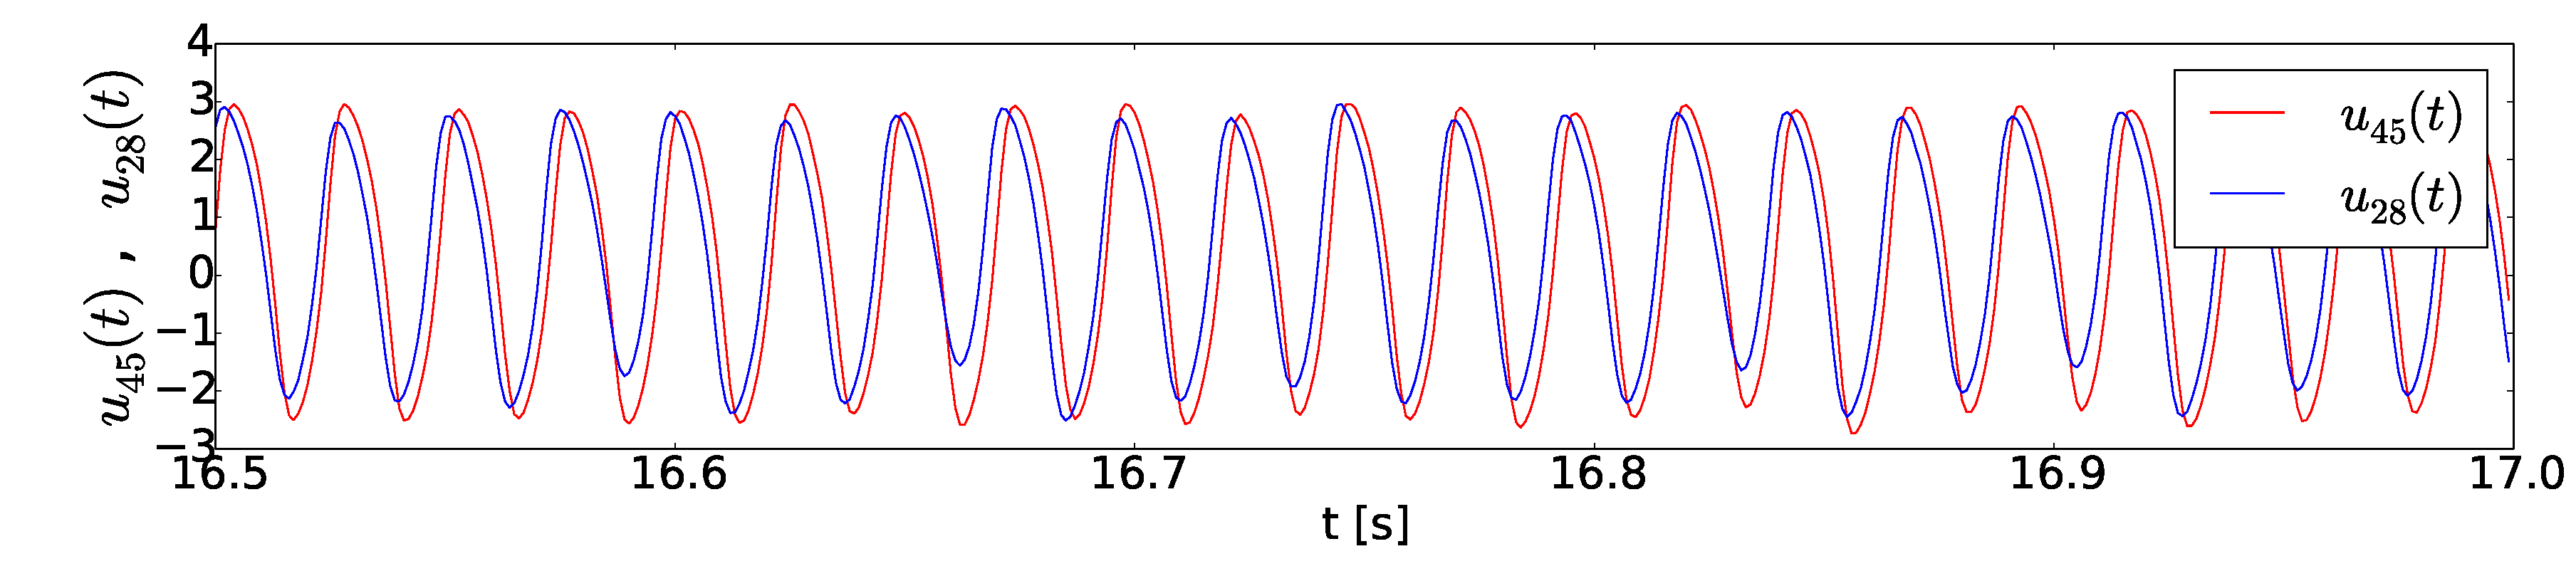
\includegraphics[width=\textwidth]{Figures/cor_FCM_sim_no_best.eps} 
   	 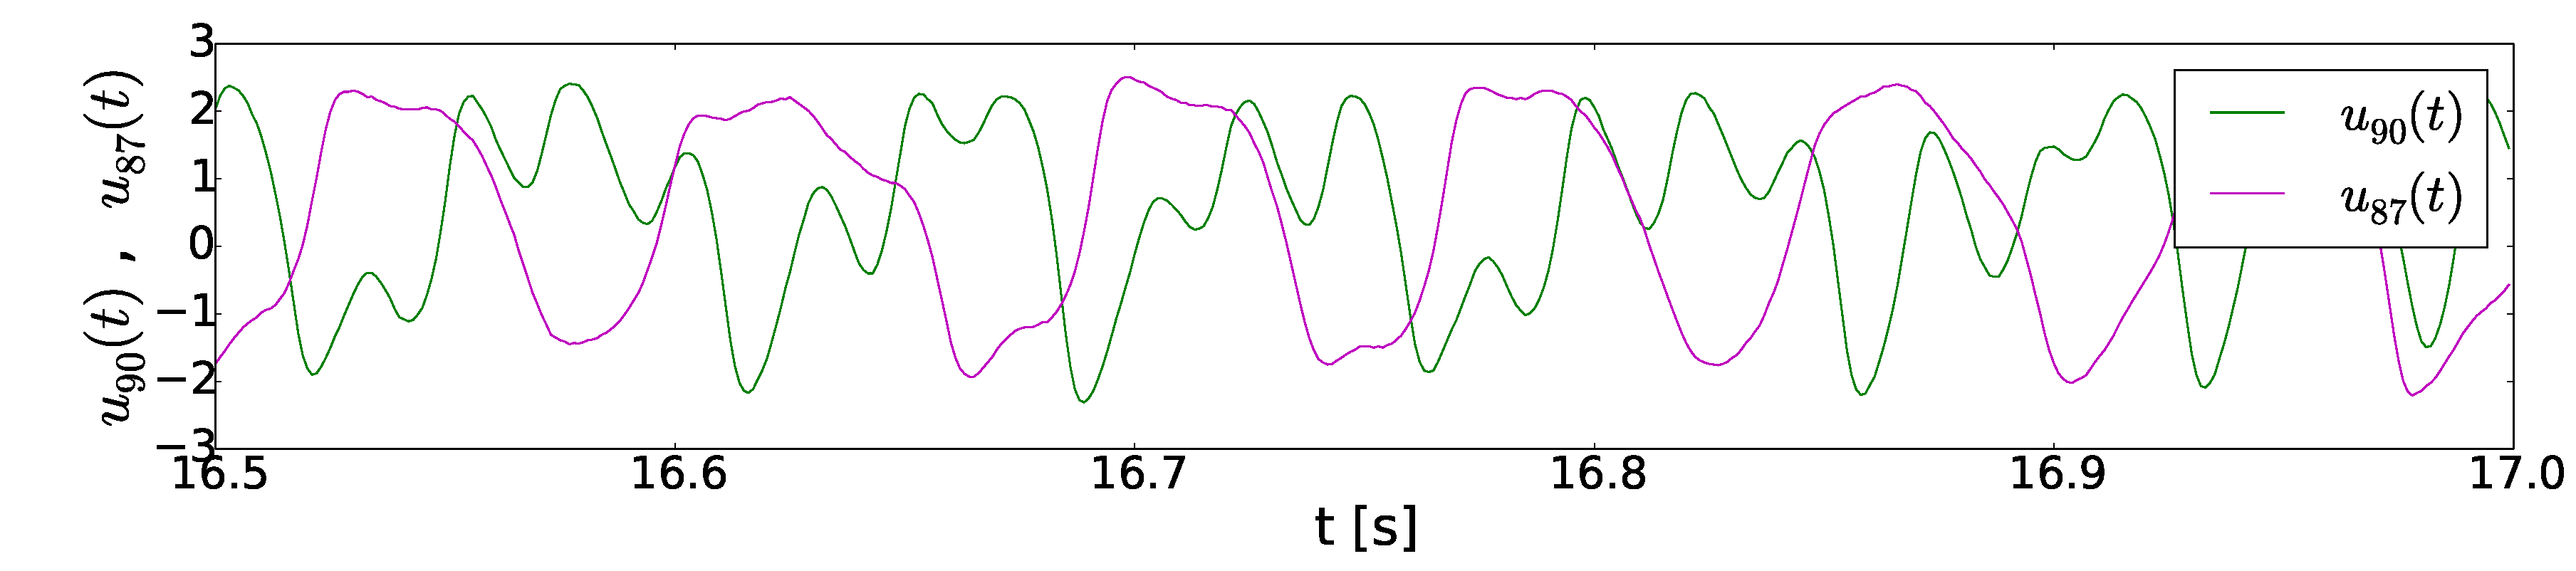
\includegraphics[width=\textwidth]{Figures/cor_FCM_sim_no_worst.eps} 

    \rule{35em}{0.5pt}
  \caption[Neural Activity Node Dynamics, FCM]{Temporal dynamics of highly (top, $\rho_{45,28}=0.88$) and poorly (bottom, $\rho_{90,87}=0.13$) correlated node couples with FHN model. The simulation parameters are $c=0.2$, $v=7$ m/s, $r=0.60$.} 
    \label{fig:Neural Activity Node Dynamics, FCM}
 	
\end{figure} 



All $\rho_{i,j}$ values among any possible pairwise combination of $N=90$ nodes are then used to built a $90\times 90$  matrix, which is referred to as simulated correlation matrix (CM). The fMRI-BOLD data was in fact used to obtain a functional correlation matrix (FCM). (Figure 2.1 , Section 2.1). Figure 3.2 illustrates a simulated CM and the empirical FCM together for a better visualization. Each colored square represents how strong any pair of nodes $i$ and $j$ addressed on $x$- and $y$-axes are correlated in terms of \textit{i)} their temporal dynamics for the simulated CM, \textit{ii)} their BOLD fluctuations for empirical FCM. Colorbars denote $\rho_{i,j}$-values.


\begin{figure}[htbp]
 
  \centering
	 \includegraphics[width=0.49\textwidth]{Figures/cor_FCM_sim.eps} 
   	 \includegraphics[width=0.49\textwidth]{Figures/cor_FCM_exp.eps} 

    \rule{35em}{0.5pt}
  \caption[High correlated FHN simulation, FCM]{ Simulated CM obtained from FHN network simulations (left) and empirical FCM (right). The parameters of CM are $c=0.2$, $v=7$ m/s, $r=0.60$, overall correlation between two matrices is $\rho_{e,s} = 0.43$}
      \label{fig:High correlated FHN simulation, FCM}
 	
\end{figure}  



In order to compare the modeling approach to the empirical result, both correlation matrices are compared statistically with Pearson's correlation coefficient, the same linear pairwise correlation method again. All correlation values $\rho_{e,s}$ between empirical $e$ and simulated $s$ data matrices are placed on the parameter spaces. Here, the parameter spaces are designed over $(r,v)$ and $(r,c)$ as seen in Figure 3.3. The purpose is to explore the most promising values for three tuning parameters : $r$, which defines the topology of AM, the coupling strength $c$ and signal propagation velocity $v$, which are parameters of the FHN model as explained in Section 2.5.  Each color coded square in Figure 3.3 corresponds to one $\rho_{e,s}$ value. Hot colors represent high correlation between simulated and empirical data, 0 means no correlation at all and cold colors below zero points out anti-correlations.


A correlation value close to 1 in FCM indicates that the quantified functional activities of corresponding nodes in the right and left hemisphere highly resemble each other, see subdiagonals in Figure 3.2 (right). The AAL regions tend to be correlated at $\rho_{i,j}=0.5$ in FCM. The simulated CM exhibit in general either higher correlations or anti-correlations, see Figure 3.2 (left). The traces of subdiagonals in FCM can be observed slightly on the simulated CM. The overall correlation between CM and FCM is $\rho_{e,s}=0.43$. 


It can be inferred from Figure 3.3 that fast signal propagation velocity $v$ above $6$ m/s, a low $r$ in the range of  $[0.54, 0.60]$ and a coupling strength $c$ around $[0.1, 0.4]$ would result in high correlations between simulated and empirical data sets. The $v$-value range was already shown to be around $7$ m/s in the previous studies \citep{VUK13, GHO08a}. The network topology of the brain graphs constructed via AM's is characterized for $r$-values, i.e. $0.54 \leq r \leq 0.60$ corresponds to a network density $  0.35 \geq  \kappa \geq 0.18 $ (Section 2.4.1). Beyond $r > 0.60$, less densely connected brain networks exhibit dramatically changing transitivity $T$, shortest pathway $d_{ij}$, small worldness $S$ and assortativity $A$ (Section 2.4 and Appendix B) and simulations become distinctly different from experiment.  


\begin{figure}[htbp]
 
  \centering
    \includegraphics[width=0.49\textwidth]{Figures/PA_FCM_c_02.eps} 
	\includegraphics[width=0.49\textwidth]{Figures/PA_FCM_v_7.eps} 

	
    \rule{35em}{0.5pt}
  \caption[Parameter Analysis, FCM]{Analogy between FHN network model simulated brain graphs obtained from FC map and fMRI-BOLD result in parameter spaces $(r,v)$ (constant coupling strength $c=0.2$, left) and $(r,c)$ (constant velocity $v=7$ m/s, right). The colorbars stand for $\rho_{e,s}$.  }
  \label{fig:Parameter Analysis, FCM}
 	
\end{figure}  


Figure 3.4 concludes this section with a fast Fourier transform analysis over all nodes given in Figure 3.2. The $z$-axis of 3D plot has a natural logarithmic scale in order to magnify the frequency power spectrum values. The FHN model results mostly in very fast oscillations around  $20$ Hz, $40$ Hz and $58$ Hz quite uniform. The slow oscillatory component peaks around $0.1$ Hz. The BOLD fluctuations are ultra slow scaled oscillations ($<0.1$ Hz), and FHN network model is not capable of capturing the BOLD activity. All extracted neuronal time-series will be used to implement the BOLD dynamics later in Section 3.2.


\begin{figure}[htbp]
 
  \centering
	 \includegraphics[width=0.8\textwidth]{Figures/FFT_FCM.eps} 
   	 %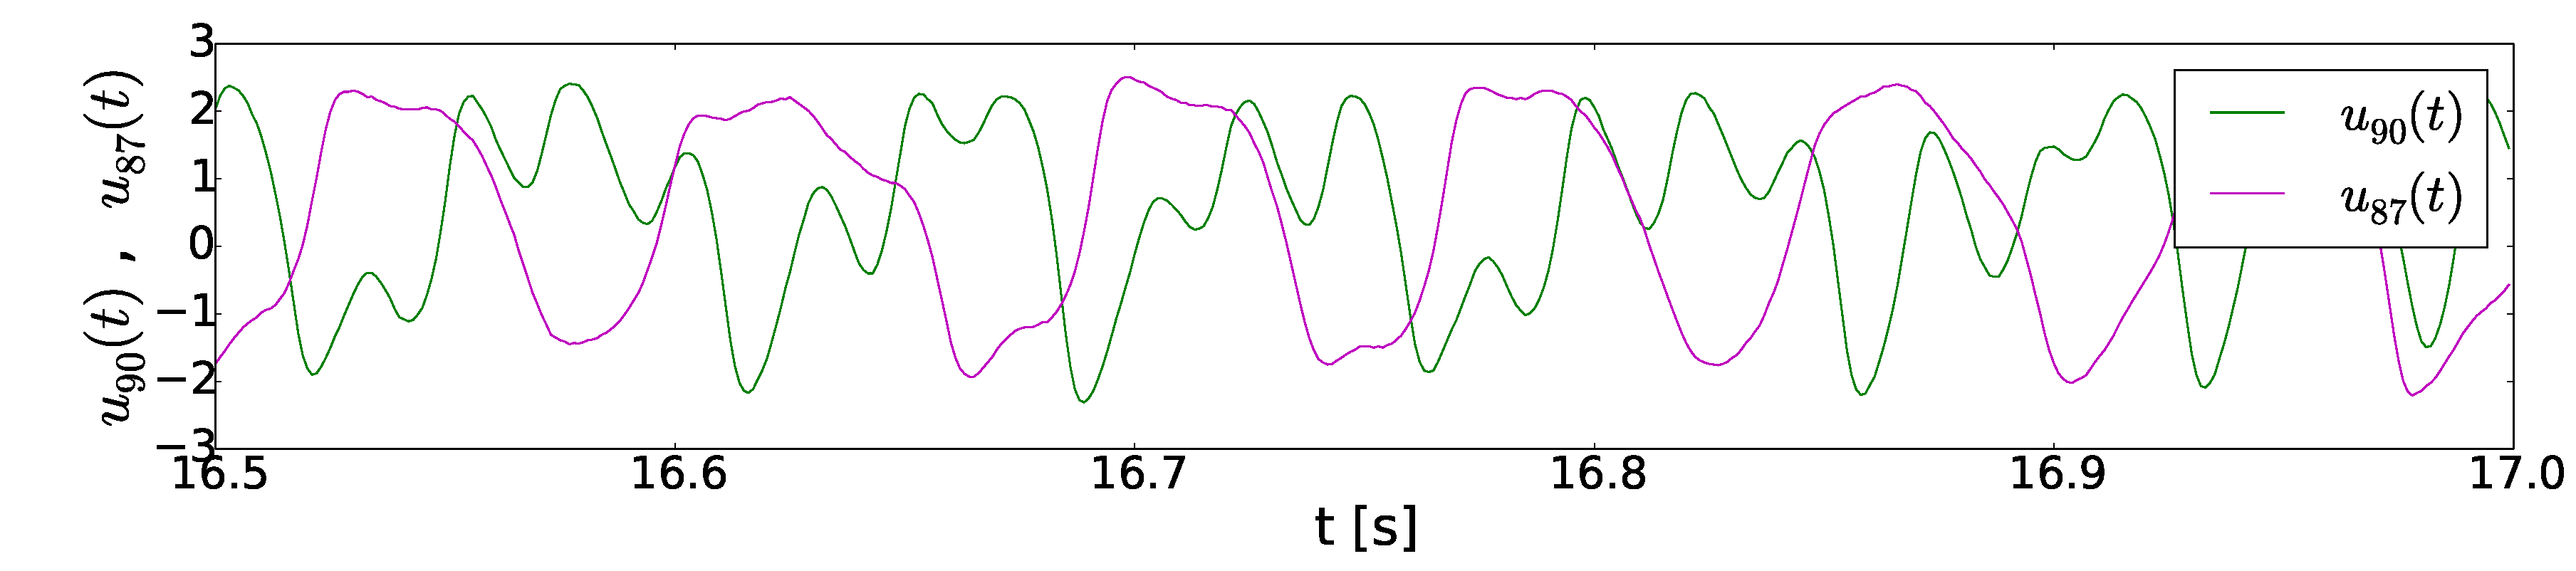
\includegraphics[width=\textwidth]{Figures/cor_FCM_sim_no_worst.eps} 

    \rule{35em}{0.5pt}
  \caption[3D Fast Fourier Transform, FHN, FCM]{Illustration of fast Fourier transform of neuronal activity oscillations corresponding to $N=90$ nodes in simulated CM with parameters given in Fig.3.2.} 
    \label{fig:3D Fast Fourier Transform, FHN, FCM}
 	
\end{figure}  

The next subsection will cover the FHN network model simulation results obtained from the anatomical brain graphs. The statistical comparison of temporal dynamics of node pairs as well as the comparison of simulated and empirical data will be quantified with the same methodology: the Pearson's correlation coefficients. 

\subsection{Anatomical Brain Graphs Compared to DW-MRI Data}

The adjacency matrix (AM) used in this subsection are constructed via binarizing the anatomical connectivity (AC) map at probability $p=[0.18, 0.82]$. AC map used in this project is obtained from the DW-MRI technique at resting-state of brain, which reveals the probability of any two AAL regions to be structurally connected with the fiber tracks (Section 2.1). The AAL nodes refer to the same cortical and sub-cortical regions used in fMRI-BOLD data extraction (Appendix A). The AM constructed via ACM represents whether or not any pair of nodes $i,j$ is structurally connected above a given $p$ (Section 2.2).  

Investing the temporal properties of the brain's AC map is done within the same methodological order as in the previous section. AM's obtained at different $p$ are simulated with the FHN network model, neural time-series $u(t)$ of each node is extracted and Pearson correlation coefficients $\rho_{i,j}$ of temporal dynamics between all pairwise combinations of nodes $i,j$ are calculated. For each FHN network model simulated on AM, a $90 \times 90$ matrix is built with calculated $\rho_{i,j}$ values. This matrix is referred to as simulated correlation matrix (CM). The simulated CM's are then compared to the empirical ACM by pairwise Pearson's correlation coefficients $\rho_{e,s}$. The results are carried in to $(p,v)$ and $(p,c)$ parameter spaces. $p$ will lead us to interpret the network topology of the brain graph. The signal velocity along the axons $v$ and the coupling strength $c$ will be used as tuning parameters of FHN model as inspired from the previous studies \citep{VUK13, GHO08a}. This subsection begins from a broad manner by demonstrating $\rho_{e,s}$-values in parameter spaces, and goes narrower into node dynamics. 

\begin{figure}[htbp]
 
  \centering
    \includegraphics[width=0.49\textwidth]{Figures/PA_ACM_c_03.eps} 
	\includegraphics[width=0.49\textwidth]{Figures/PA_ACM_v_6.eps} 

	
    \rule{35em}{0.5pt}
  \caption[Parameter Analysis, ACM]{Analogy between FHN network model simulated brain graphs derived from AC map and DW-MRI result in parameter spaces $(r,v)$ (constant coupling strength $c=0.3$, left) and $(r,c)$ (constant velocity $v=6$ m/s, right). The colorbars stand for $\rho_{e,s}$.}
  \label{fig:Parameter Analysis, ACM}
 	
\end{figure}       

Figure 3.5 illustrates Pearson coefficients $\rho_{e,s}$ between experimental $e$ and simulated $s$ correlation matrices in parameter spaces. Highest correlation regime is captured at $4$m/s$<v<8$m/s, $0.1 < c \leq 0.5$ with $0.18 \leq p \leq 0.70 $. The network density of brain graphs based on AC map is $0.35 \geq   \kappa \geq 0.18$ for the corresponding $0.18 \leq p \leq 0.70 $ (Section 2.4.1). The pattern of $\rho_{e,s}$-values in Figure 3.5 and Figure 3.3 (Section 3.1.1) resembles each other. 

$p$ of ACM's lies in a broader range than $r$ of FCM's, when Figure 3.5 is compared to Figure 3.3. The network measures of AC map based brain graphs change smoothly with $0.18<p<0.82$, whereas that of FC map related brain graphs change sharply with $0.18<r<0.82$. This is why larger steps binarization steps by amount of 0.4 are used. However, at $p>0.82$ AC map related brain networks tend to have sudden changes in transitivity $T$, shortest pathway $d_{ij}$, small worldness $S$  and assortativity $A$. (All network measures related to the brain graphs can be reviewed through Section 2.4 and Appendix B.)

\begin{figure}[htbp]
 
  \centering
	 \includegraphics[width=0.49\textwidth]{Figures/cor_ACM_sim.eps} 
   	 \includegraphics[width=0.49\textwidth]{Figures/cor_ACM_exp.eps} 

    \rule{35em}{0.5pt}
  \caption[High correlated FHN simulation, ACM]{ Simulated CM obtained from FHN network simulations (left) and empirical FCM (right). The parameters of CM are $c=0.3$, $v=6$ m/s, $r=0.50$, overall correlation between two matrices is $\rho_{e,s} = 0.43$ }
    \label{fig:High correlated FHN simulation, ACM}
 	
\end{figure}

Figure 3.6 illustrates a simulated CM (left) together with the empirical ACM (right). The simulated CM is chosen from the red-colored squares in Figure 3.5, for instance, the illustrated matrices in Figure 3.6 has a correlation value of $\rho_{e,s}=0.43$. The hot colors in the simulated CM present highly correlating node pairs in terms of their simulated neuronal time-series, whereas the cold colors express poor correlations. It should be noted that only the excitator variable $x$ of FHN model is considered to quantify correlations (Section 2.5). The colorbar of the empirical ACM denotes the probability $p$ values of two nodes to be connected via nerve fibers.
 
Figure 3.6 indicates that the nodes in the same hemispheres are more probably to be connected via fiber tracts, see two dominating subsquares in the empirical ACM. The FHN network model simulated on the anatomical brain graph yields also highly correlated temporal activities for the nodes in the same sphere, see subsquares in the simulated CM. However, the correlations of neuronal time-series in CM tend to be more pronounced in comparison to the anatomical connectivity probabilities in the empirical ACM. Although some node pairs are not structurally connected at all, they are captured to be functionally connected via their extracted FHN time-series.  

Choosing one red square and one blue square from the simulated CM in Figure 3.6, the simulated time-series of highly and poorly synchronizing node pairs are visualized in Figure 3.7. The modeled temporal dynamics of nodes 43 and 31 are highly correlated, $\rho_{43,31}=0.86$, whereas that of nodes 90 and 83 are poorly correlated $\rho_{90,83}=0.15$.

\begin{figure}[htbp]
 
  \centering
	 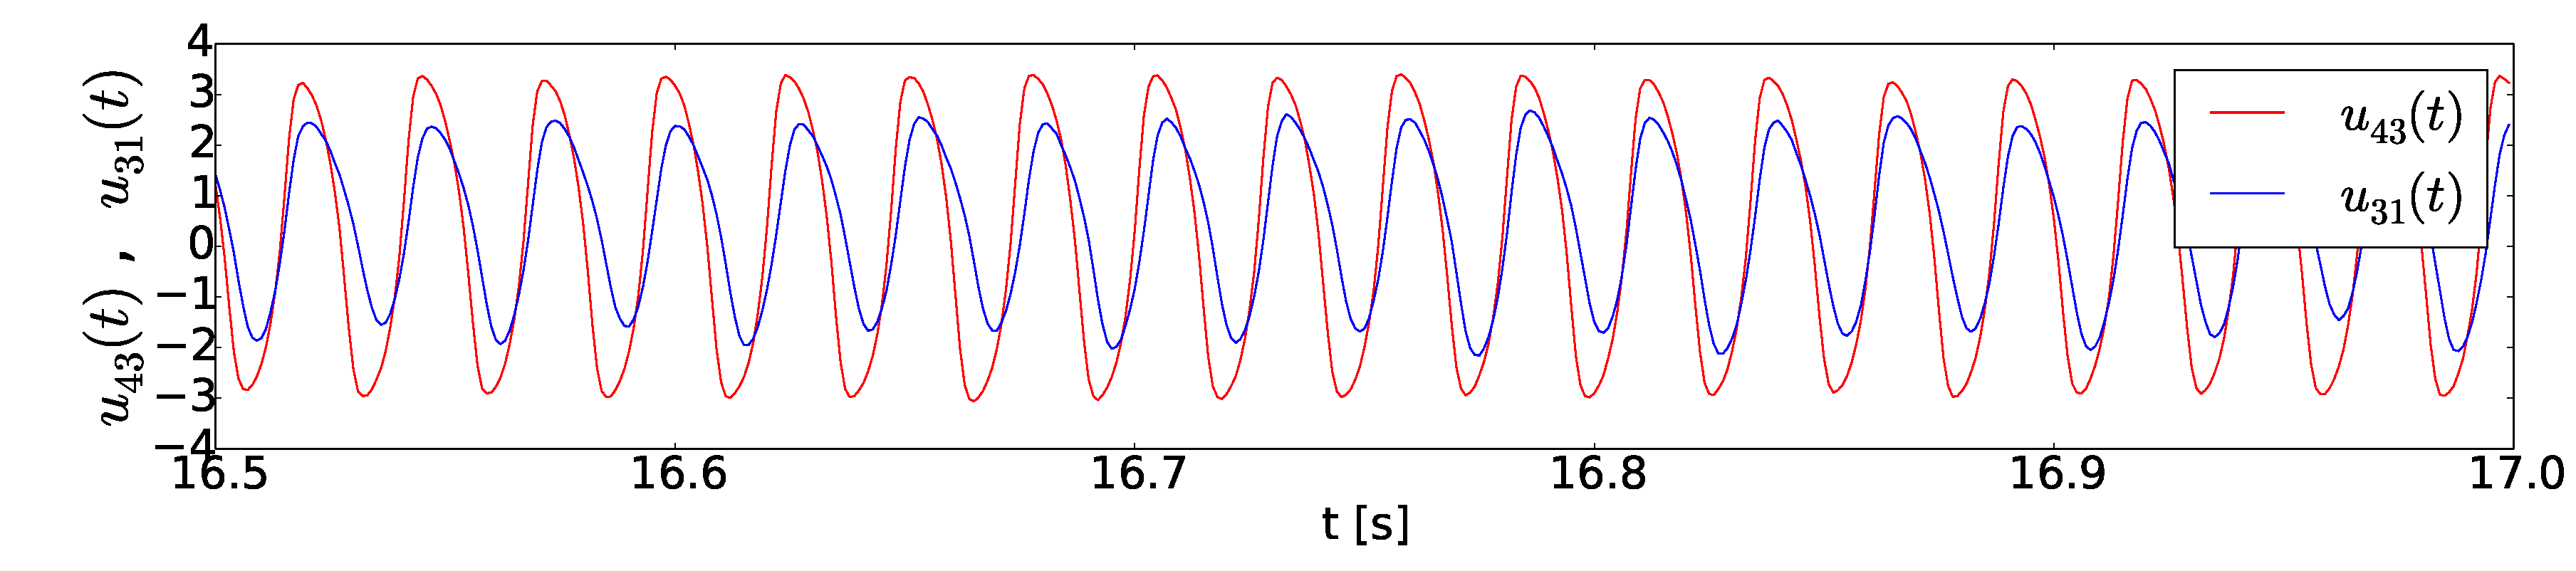
\includegraphics[width=\textwidth]{Figures/cor_ACM_sim_no_best.eps} 
   	 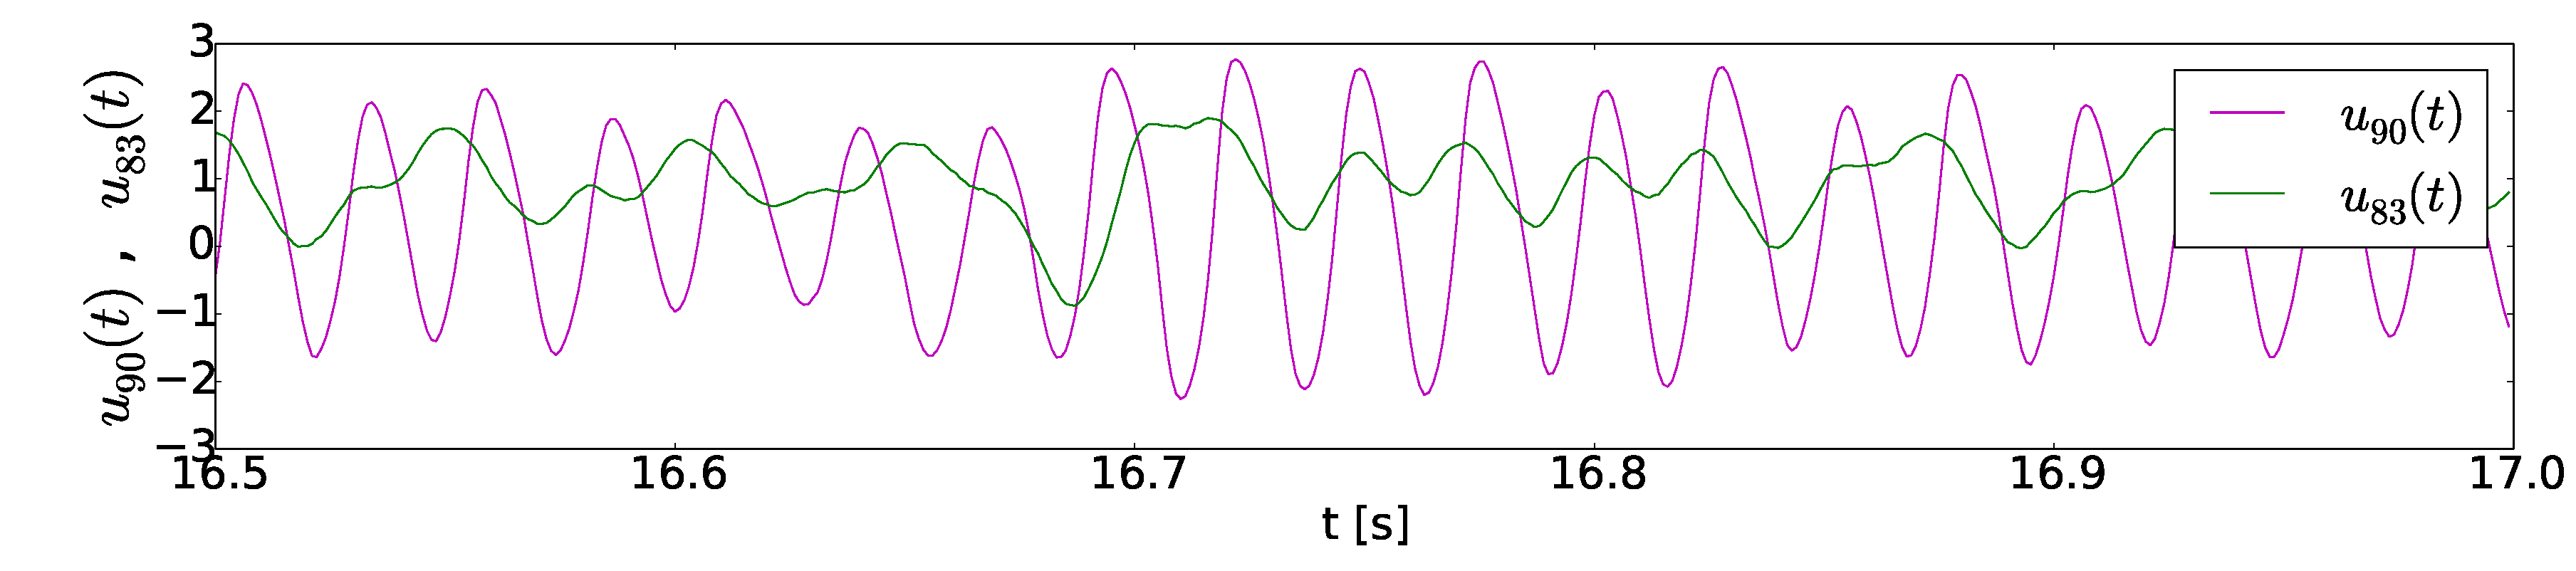
\includegraphics[width=\textwidth]{Figures/cor_ACM_sim_no_worst.eps} 

    \rule{35em}{0.5pt}
  \caption[Neural Activity Node Dynamics, ACM]{ Temporal dynamics of highly (top, $\rho_{43,31}=0.86$) and poorly (bottom, $\rho_{90,83}=0.15$) correlated node couples with the FHN model. The simulation parameters are $c=0.3$, $v=6$ m/s, $r=0.50$.} 
    \label{fig:Neural Activity Node Dynamics, ACM}
 	
\end{figure} 

Finally, a fast Fourier transform (FFT) is carried out to identify the dominating frequency $\nu$-ranges of the FHN network model oscillations. All $N=90$ nodes of the simulated CM given in Figure 3.6 (left) are analyzed with FFT in Figure 3.8. The temporal dynamics of the nodes are fast oscillatory at $40$ Hz $< \nu < 60$ Hz, a slow oscillatory peak is observed around $\nu = 0.1 [Hz]$. The frequency scale of oscillations are in agreement in Figures 3.8 and 3.4. However, the scale of BOLD fluctuations is extremely small compared to the modeled temporal dynamics. 



\begin{figure}[htbp]
 
  \centering
	 \includegraphics[width=0.8\textwidth]{Figures/FFT_ACM.eps} 
   	 %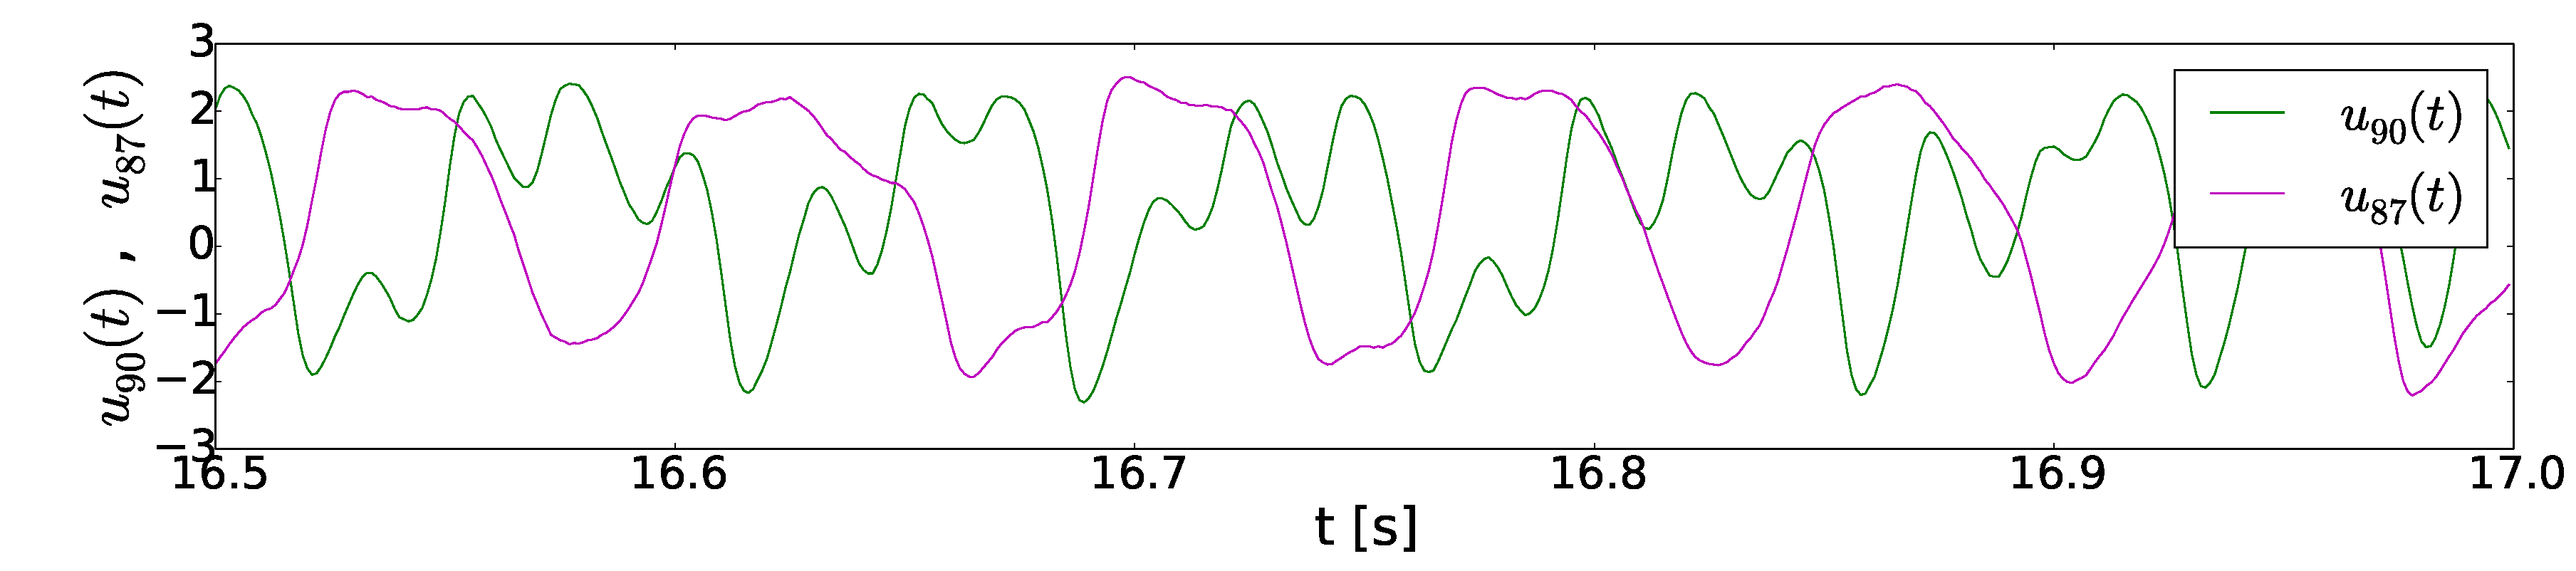
\includegraphics[width=\textwidth]{Figures/cor_FCM_sim_no_worst.eps} 

    \rule{35em}{0.5pt}
  \caption[3D Fast Fourier Transform, FHN, ACM]{Illustration of fast Fourier transform of neuronal activity oscillations corresponding to $N=90$ nodes in simulated CM with parameters given in Figure 3.6.} 
    \label{fig:3D Fast Fourier Transform, FHN, ACM}
 	
\end{figure}  

Up to here, the neuronal activity model of human brain at the resting-state is built on FitzHugh-Nagumo oscillatory network model as previously proposed in \citep{VUK13, GHO08a} (Section 2.5). This model is applied to the adjacency matrices obtained from functional and structural connectivity maps, which are derived from fMRI-BOLD and DW-MRI measurements, respectively. Each FHN network model simulated brain graph (derived from FC and AC maps) compared to their original data sets (empirical FCM and ACM). High correlations between the FHN network model simulations and experimental data sets are captured on parameter spaces by tuning model parameters of $c$ and $v$, as well as network topology parameter $p$ or $r$ \citep{VUK13, GHO08a}. The next step is to model the low frequency oscillating BOLD activity ($<0.1$ Hz) of resting-state by using the extracted neuronal time-series. The next section will demonstrate the modeled BOLD activity by using theses neuronal time-series. 


\section{BOLD Activity Simulations}

Blood oxygen level dependent (BOLD) contrast imaging is one of the underlying mechanisms of fMRI to map the functional activity correlations among brain regions at the resting-state. The existing models of resting-state brain dynamics hypothesize that functional interactions result from a complex interplay between intrinsic brain dynamics and underlying structural connections \citep{RUB09}. One of the research objectives of this Master's project is to investigate whether it is possible to capture the BOLD signal through the anatomical connectivity map provided by DW-MRI technique. The BOLD activity here is inferred via the Baloon-Windkessel hemodynamic model \citep{FRI00}(Section 2.6). The input of this model is the simulated neuronal activity (Section 2.5), and the output is designed to be a hemodynamic oscillation ($<0.1$ Hz) analogous to the BOLD signal (Section 2.6) \citep{FRI00}. The previous section already demonstrated the FitzHugh-Nagumo network model results for the temporal dynamics of brain nodes at the resting-state \citep{VUK13, GHO08a}, and this section feeds the extracted time-series into the BOLD activity model. 

The extracted time-series for the neuronal activity are chosen from right-hand sides of Figure 3.3 and Figure 3.5, corresponding to the FHN network model simulations of functional and anatomical brain networks in the respective $(c,r)$ and $(c,p)$ parameter spaces. All time-series are normalized around their mean values and then embedded to the hemodynamic model. The comparison of simulated BOLD activity to the empirical fMRI-BOLD data is quantified statistically with the same methodological order as in Section 3.1 : \textit{i)} the correlations $\rho_{i,j}$ of the simulated BOLD oscillations of any node pairs $i,j$ among $N=90$ nodes are calculated via Pearson's coefficients, \textit{ii)} a simulated correlation matrix (CM) of size $90 \times 90$ is constructed with all $\rho_{ij}$ values, \textit{iii)} the simulated CM is compared to the empirical functional correlation matrix (FCM) derived from fMRI-BOLD measurement via Pearson's statistical approach again.    


\begin{figure}[htbp]
 
  \centering
    \includegraphics[width=0.49\textwidth]{Figures/PA_BOLD_FCM_v_7.eps} 
	\includegraphics[width=0.49\textwidth]{Figures/PA_BOLD_ACM_v_3.eps} 

	
    \rule{35em}{0.5pt}
  \caption[Parameter Analysis, BOLD]{Parameter analysis for the comparison of fMRI-BOLD data to the modeled BOLD activity on the functional (constant signal propagation velocity $v=7$ m/s, left) and on the anatomical brain graphs (constant $v$=3 m/s, right). }
  \label{fig:Parameter Analysis, BOLD}
 	
\end{figure} 

Figure 3.9 illustrates statistical comparisons between simulated CM's and  the experimental FCM of the BOLD activity. The input of the modeled BOLD activity is the neuronal time-series extracted from functional (Figure 3.9, left) and anatomical (Figure 3.9, right) brain networks (Sections 2.1 and 2.2). The colorbars represent Pearson correlation coefficients $\rho_{e,s}$ between empirical $e$ and simulated $s$ correlation matrices. 

In Figure 3.9, the BOLD activity simulations tend to be in better agreement with the empirical FCM at low coupling strength $c \leq 0.1$ for both anatomical and functional brain networks. It can be inferred that, the smaller scaled the neuronal activity oscillations are, the higher correlation between the BOLD simulations and fMRI-BOLD data is captured. The anatomical brain networks exhibit a finer correlation pattern compared to the functional brain networks. It is possible to capture functional BOLD fluctuations observed in fMRI at the resting-state through the structural connectivity of the brain, especially at low coupling strength $c$, a low axonal propagation velocity $v=3$ m/s and $p<0.70$ (hot colors in Figure 3.9, right). 

The network topology of anatomical brain graphs has a more pronounced effect for the $\rho_{e,s}$ values in comparison to that of functional brain graph. $0.18<p<0.70$ corresponds to very smoothly changing network measurements in the brain graphs obtained from DW-MRI data (Section 2.4, Appendix B). Figure 3.9 (left) does not have a well-interpreted $\rho_{e,s}$-pattern in the $(r,c)$ parameter space. $0.54<r<0.66$ corresponds to sharply changing network properties in the functional brain graphs. The $\rho_{e,s}$-values in Figure 3.9 (left) are mostly around zero or weak correlation.



\begin{figure}[htbp]
 
  \centering
	 \includegraphics[width=0.49\textwidth]{Figures/cor_BOLD_FCM_sim.eps} 
   	 \includegraphics[width=0.49\textwidth]{Figures/cor_FCM_exp.eps} 

    \rule{35em}{0.5pt}
  \caption[Well correlated BOLD simulation, FCM]{Correlated BOLD activity simulation of functional brain graph with $c=0.03$, $v=7$ m/s and $r=0.66$ (left) and empirical FCM derived from fMRI-BOLD technique, $\rho_{e,s} = 0.24$.} 
    \label{fig:High correlated BOLD simulation, FCM}
 	
\end{figure}  



Figures 3.10 demonstrates the simulated CM of BOLD activity extracted from functional brain graph together with the empirical (FCM) obtained from fMRI-BOLD technique. The simulated CM is chosen from green/orange-colored parameters in Figure 3.9 (left). The Pearson correlation coefficient between the simulated CM and the empirical FCM is $\rho_{e,s} = 0.24$. This is a relatively low correlation coefficient compared to the $\rho_{e,s}$-values captured for the simulated neuronal activity in Section 3.1.

In Figure 3.10, the trace of subdiagonals in the empirical FCM is lost in the simulated CM. However, both matrices have common neuronal populations (or brain nodes) in the left and right hemispheres, whose correlated BOLD activity tend to be almost equivalently strong, see hot colored subsquares in simulated CM and FCM.



\begin{figure}[htbp]
 
  \centering
	 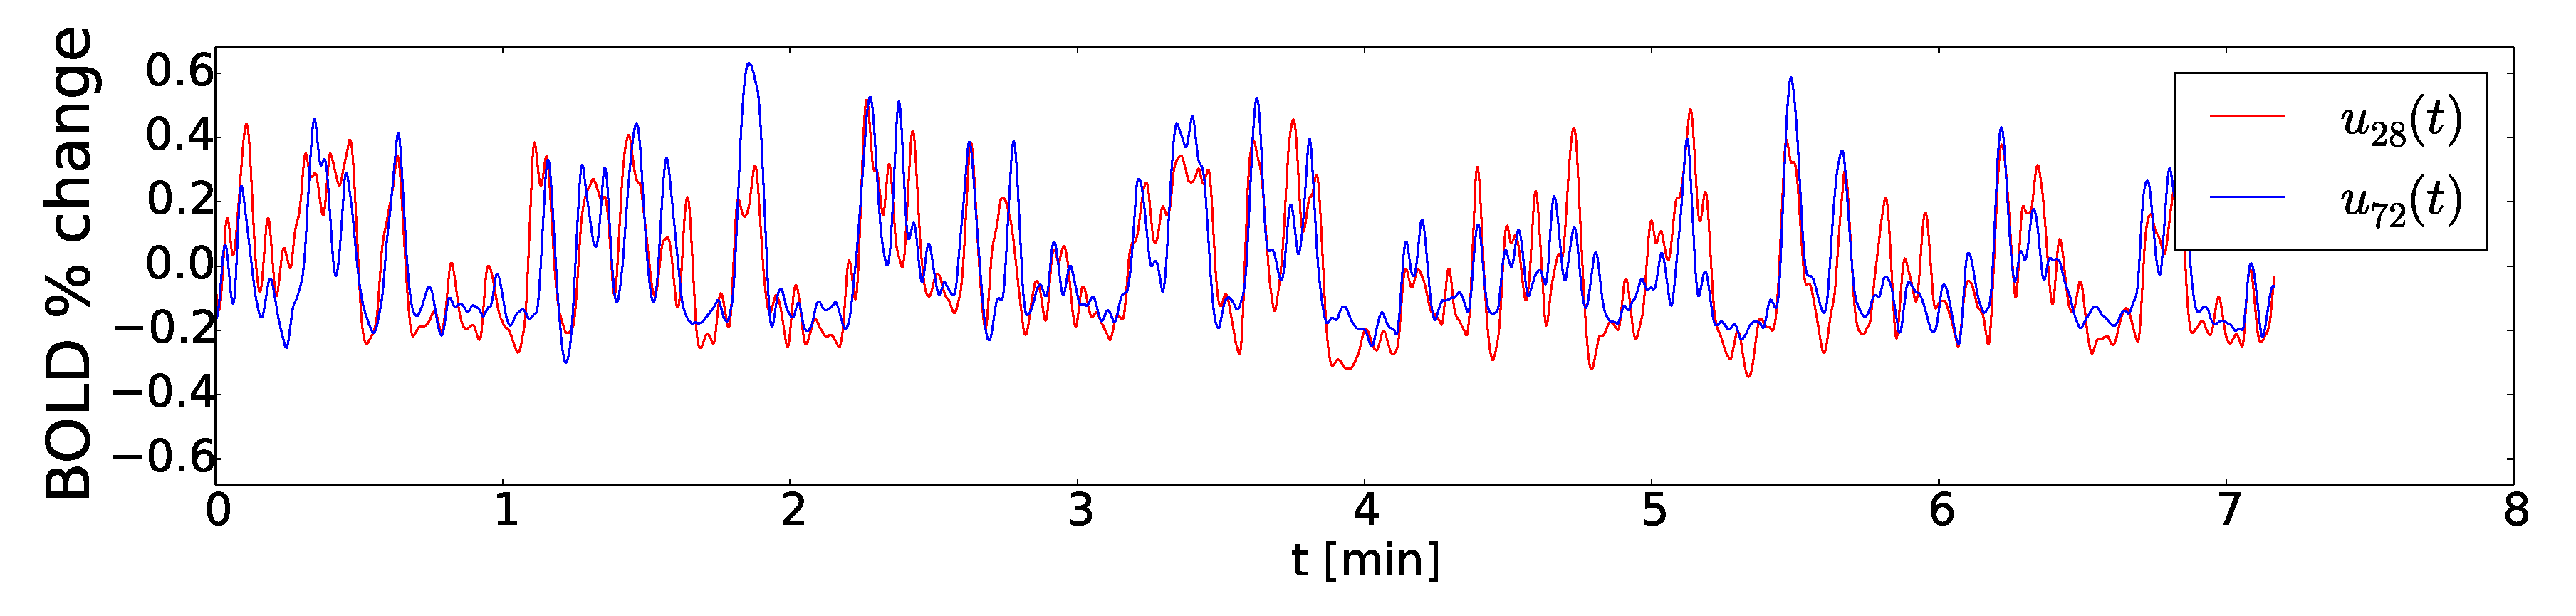
\includegraphics[width=\textwidth]{Figures/cor_BOLD_FCM_sim_no_best.eps} 
   	 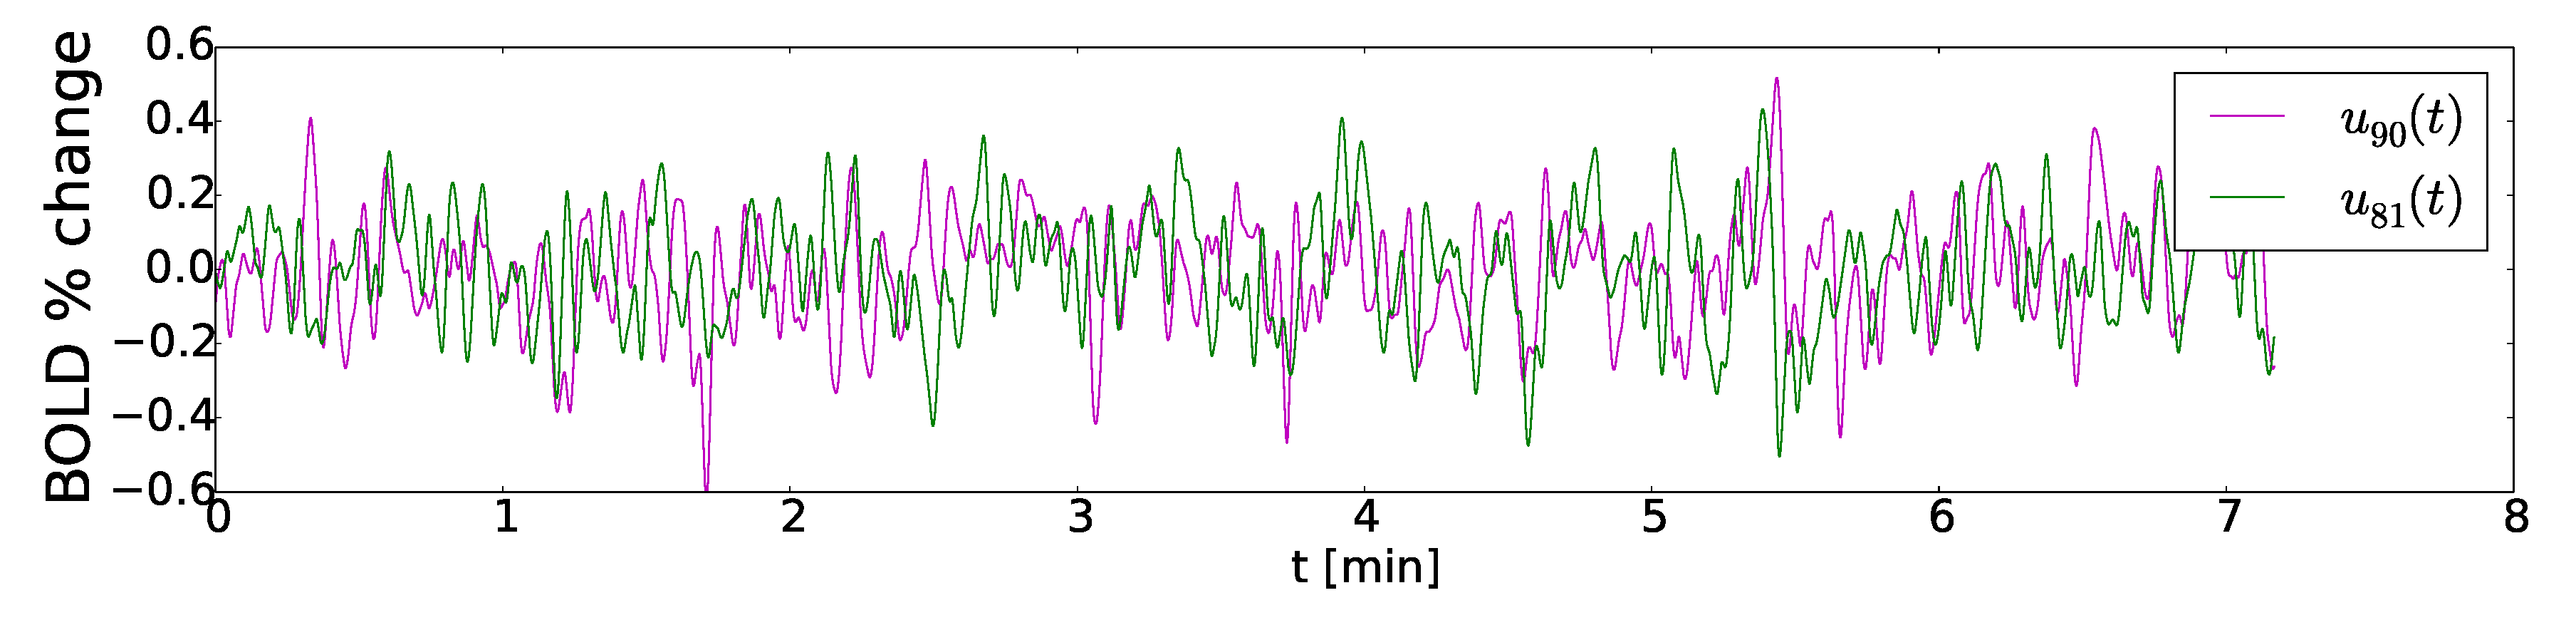
\includegraphics[width=\textwidth]{Figures/cor_BOLD_FCM_sim_no_worst.eps} 

    \rule{35em}{0.5pt}
  \caption[BOLD Activity Node Dynamics, FCM]{Simulated BOLD activity of highly (top, $\rho_{28,72}=0.75$) and poorly (bottom, $\rho_{90,81}=0.10$) correlated node couples. Both nodes are chosen from the simulated CM in Figure 3.10 ($c=0.03$, $v=7$ m/s, $r=0.66$).} 
    \label{fig:BOLD Activity Node Dynamics, FCM}
 	
\end{figure} 

Figure 3.11 illustrates temporal dynamics of the simulated BOLD activity of two node pairs. The extracted BOLD oscillations of nodes 28 and 72 are synchronized, $\rho_{28,72}=0.75$. The BOLD fluctuation of nodes 90 and 81 are poorly correlated, $\rho_{90,81}=0.10$. These node couples are chosen from hot and cold color parameters in Figure 3.10 (left).

\begin{figure}[htbp]
 
  \centering
	 \includegraphics[width=0.49\textwidth]{Figures/cor_BOLD_ACM_sim.eps} 
   	 \includegraphics[width=0.49\textwidth]{Figures/cor_FCM_exp.eps} 

    \rule{35em}{0.5pt}
  \caption[High correlated BOLD simulation, ACM]{Correlated BOLD activity simulation of anatomical brain graph with $c=0.03$, $v=3$ m/s and $p=0.54$ (left) and empirical FCM derived from fMRI-BOLD technique, $\rho_{e,s} = 0.22$.} 
    \label{fig:High correlated BOLD simulation, ACM}
 	
\end{figure}  

Figures 3.12 illustrates the simulated CM of BOLD activity extracted from anatomical brain graph (left) together with the empirical (FCM) obtained from fMRI-BOLD measurement (right). The simulated CM is chosen from red/orange-colored parameters in Figure 3.9 (right). The Pearson correlation coefficient between the simulated CM and the empirical FCM is $\rho_{e,s} = 0.22$. This is again a relatively low correlation coefficient compared to Section 3.1. 

In Figure 3.12, the trace of subdiagonals in the empirical FCM is almost lost in the simulated CM. The nodes in right and left hemispheres correlate around $\rho_{i,j}=0.1$ in the simulated CM (yellowish subdiagonals on CM), while they are highly correlated empirically (red subdiagonals in FCM). The correlations between node pairs located in left-left, right-right, left-right and right-left can be distinguished in both CM and FCM. Both matrices have distinct neuronal populations (or brain nodes), whose correlated BOLD activity tend to be high, see hot-colored subsquares in Figure 3.12. However, these subpopulations do not refer exactly to the same AAL regions in CM and in FCM, but they are at least on the same hemisphere. 

\begin{figure}[htbp]
 
  \centering
	 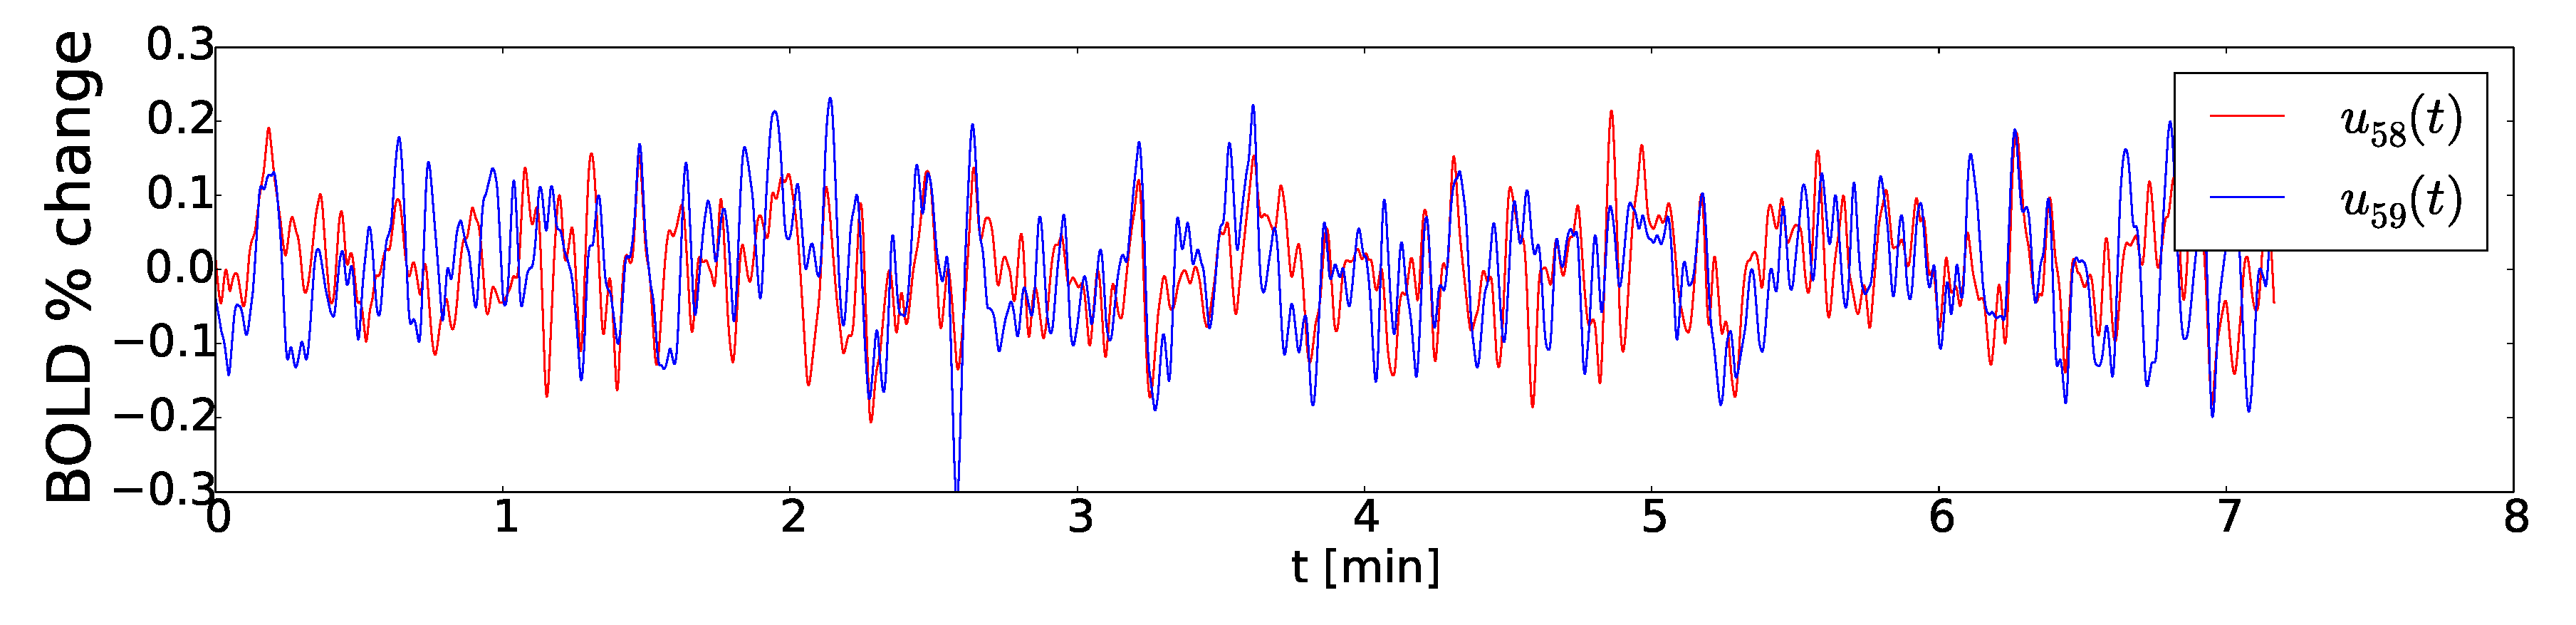
\includegraphics[width=\textwidth]{Figures/cor_BOLD_ACM_sim_no_best.eps} 
   	 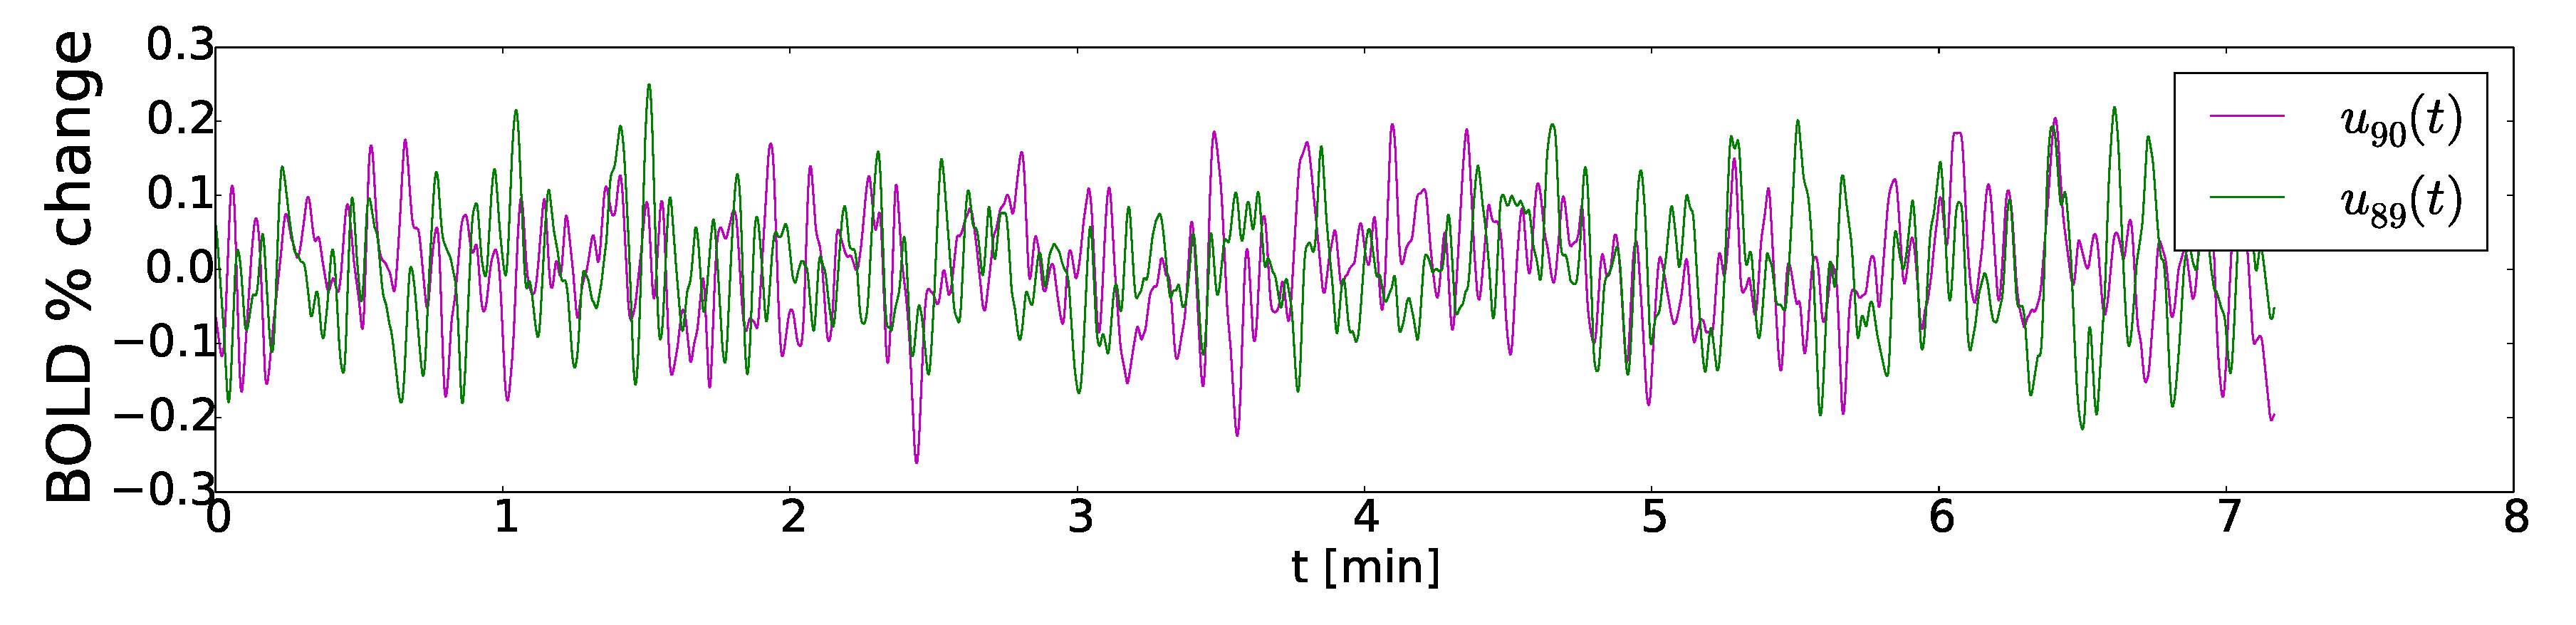
\includegraphics[width=\textwidth]{Figures/cor_BOLD_ACM_sim_no_worst.eps} 

    \rule{35em}{0.5pt}
  \caption[BOLD Activity Node Dynamics, ACM]{Simulated BOLD activity of highly (top, $\rho_{58,59}=0.48$) and poorly (bottom, $\rho_{90,89}=0.11$) correlated node couples. Both nodes are chosen from the simulated CM in Figure 3.12 ($c=0.03$, $v=3$ m/s, $p=0.54$).} 
    \label{fig:BOLD Activity Node Dynamics, ACM}
 	
\end{figure} 



Figure 3.13 demonstrates temporal dynamics of the simulated BOLD activity of two node pairs chosen from anatomical brain graph. The extracted BOLD oscillations of nodes 58 and 59 are synchronized, $\rho_{58,59}=0.48$. The BOLD fluctuation of nodes 90 and 89 are poorly correlated, $\rho_{90,89}=0.11$. These node couples are chosen from hot and cold color parameters from the simulated CM in Figure 3.12 (left).

This subsection closes with a fast Fourier transform analysis performed for the oscillation frequencies $\nu$ of simulated BOLD activity model on functional and brain graphs. The simulated CM's visualized in Figure 3.10 and 3.12 are chosen as exemplary simulated brain connectivity maps at the resting-state. Figure 3.14 visualizes the pronounced $\nu$-ranges identified for all $N=90$ nodes in functional (top) and anatomical brain graphs (bottom). The power spectrum indicates that, BOLD fluctuations are dominant around $\nu =0.1$ Hz and they are uniform over all nodes. The $\nu$-range on the $x$-axis is limited to 2 Hz, since there is no higher $\nu$ than 2 Hz is observed for the BOLD activity simulations. 

Given a fast oscillating neuronal time-series as the input, the Balloon-Windkessel hemodynamic model \citep{FRI00} acts on it as a low-pass filter. The resulting fluctuations are ultra slow in the frequency range. This section showed that the modeled hemodynamic model resulted in plausible BOLD oscillations around 0.1 Hz. It is possible to capture the traces of BOLD fluctuations by modeling the structural connectivity map of the brain (Figure 3.9, left). However, the simulated CM's of BOLD activity are not yet fully in agreement with the empirical FCM (Figure 3.9, 3.10 and 3.12). The Ballon-Windkessel model in Friston et al. was not designed for the resting-state dynamics of the brain \citep{FRI00}. The hemodynamic model can be further investigated with a better resting-state adaptations, i.e. its standard parameters could be recovered for the resting-state. Another approach would be analyzing the low coupled ($c\leq 0.1$) FitzHugh-Nagumo oscillators in a broader manner to provide more plausible time-series input to the BOLD model.   


\begin{figure}[htbp]
 
  \centering
	 \includegraphics[width=0.70\textwidth]{Figures/FFT_BOLD_FCM.eps} 
   	 \includegraphics[width=0.70\textwidth]{Figures/FFT_BOLD_ACM.eps}  

    \rule{35em}{0.5pt}
  \caption[3D Fast Fourier Transform, BOLD, FCM]{Illustration of fast Fourier transform of simulated BOLD activity oscillations corresponding to $N=90$ nodes in functional (top) and anatomical (bottom) brain graphs.  } 
    \label{fig:3D Fast Fourier Transform, BOLD, FCM}
 	
\end{figure}  


\section{Comparison of Brain Graphs to Random Graphs}

This section implements methods drawn from graph theory/network science in order to investigate the spatial and temporal dynamics of human brain at resting-state. The brain graphs $R_{BG}$ are constructed on the functional and anatomical connectivity maps derived from fMRI-BOLD and DW-MRI measurements, respectively (Section 2.1 and 2.2). The spatial dynamics of each network is identified in dependence on the threshold level $r$ for the functional connectivity (FC) and on the probability level $p$ for the anatomical connectivity (AM) maps of the brain. In particular, I aim to explore such conditions that distinguish the modeled neuronal activity of brain graphs from that of random networks. The random graphs are built with five randomization procedures : Erd\H{o}s-R\'{e}nyi $R_{ER}$, double-edge-swap $R_{DES}$, preserved-degree-distribution $R_{PDD}$, configuration model $R_{CM}$ and partial randomization $R_{PR}$ methods (Section 2.3, Table 2.1).  

The neuronal activity of $N=90$ AAL nodes in each network is modeled via FitzHugh-Nagumo (FHN) oscillators \citep{VUK13, GHO08a} (Section 2.5). The Pearson correlation coefficients $\rho$ between any pairwise combinations of $N=90$ nodes are calculated for the extracted neuronal time-series. These correlation coefficients are then distributed in histogram for each network at the corresponding $r$ or $p$ values and FHN parameters.

Figure 3.15 demonstrates an exemplary couple of histograms. The correlations between all possible pairwise correlations among $N=90$ time-series is $ 0 \leq \rho \leq 1$ on the $x$-axis. The number of paired nodes, whose correlations fell into a defined $\rho$-range, is normalized on the $y$-axis. FC map related $R_{BG}$ histogram (Figure 3.15, left) resembles a uniform distribution around 0, meaning dominant no-correlations among neural time-series. AC map related $R_{BG}$  histogram (Figure 3.15, right) has more frequently correlated time-series observed with $\rho$-values close to 1.0.  


\begin{figure}[htbp]
 
  \centering
	 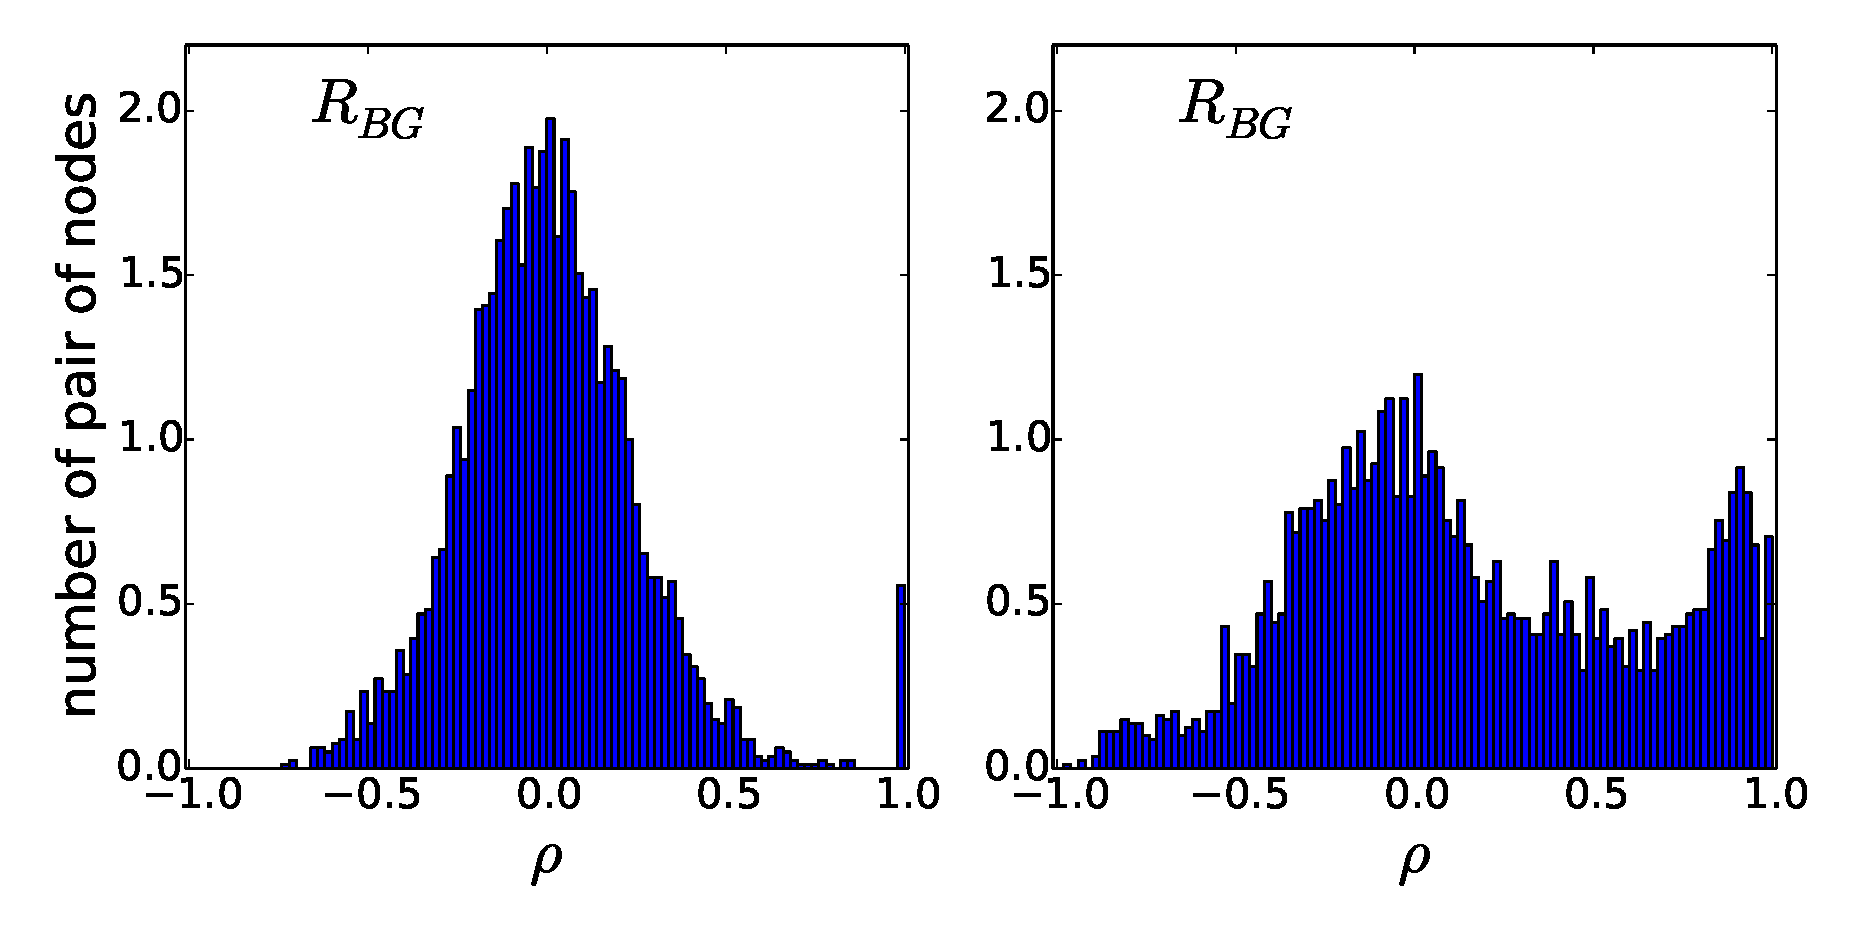
\includegraphics[width=0.8\textwidth]{Figures/sample_histo.eps}
	 \rule{35em}{0.5pt}
  \caption[Sample Histogram for Brain Graph]{Histograms for the distribution of Pearson correlation coefficients $\rho$  among all possible pairwise combinations of nodes. On the left: $R_{BG}$ obtained from FC map at $r=0.61$, FHN model parameters $c=0.1$, $v=7$ m/s. On the right: $R_{BG}$ obtained from AC map at $p=0.42$, FHN model parameters $c=0.5$, $v=6$ m/s. } 
    \label{fig:Sample Histogram for Brain Graph}
 	
\end{figure}  


Investigating the analogy between random and brain graphs requires another statistical approach than Pearson's analysis, since both graph types are not identical in terms of their network topology. The degree of similarity between brain graphs and random networks is quantified with 
Bhattacharya coefficients, a widely used statistical approach to measure the correlation between statistical samples, i.e. histograms \citep{XYZ43}. Let us denote the $\rho$ distributions of simulated neuronal activity of a brain graph with $H_b$ and that of random graph with $H_r$, the Bhattacharya coefficient $d(H_b, H_r)$ is given by the following equation:

\begin{equation}
d(H_b, H_r) = \sqrt{1- \dfrac{1}{ \sqrt{\bar{H_r} \bar{H_b} N^2}} \sum_{i} \sqrt{H_r(i)H_b(i)} } ,
\end{equation}

where $\bar{H}$ denotes the mean of histogram \citep{XYZ43}. $d(H_b, H_r)$ is scaled between 0 and 1. A high $d(H_b, H_r)$ value indicates a low correlation between $H_b$ and $H_r$, whereas a low   $d(H_b, H_r)$ value expresses a high degree of similarity. 

Brain graphs derived from \textit{i)} FC map and \textit{ii)} AC map are compared to the random networks separately as demonstrated in the next two subsections. Bhattacharya coefficients are used to quantify the analogy between brain and random graphs. The purpose is to investigate high $d(H_b, H_r)$ values indicating a diversity between brain and random graphs in the $(r,c)$ parameter spaces, where $c$ is the coupling strength for the functionally interacting nodes (Section 2.5).    


\subsection{Comparing Functional Brain Graph to the Random Graphs}

The fMRI-BOLD functional connectivity (FC) map is binarized via thresholding at $0.54 \leq r \leq 0.66$ range by step size of 0.01. An adjacency matrix (AM) is obtained for each $r$-value, indicating functionally connected node pairs with 1's and unconnected pairs with 0's (Section 2.2). AM's are used as the principal matrix structure to construct the brain graphs $R_{BG}$ with \textsc{NetworkX} tool (Section 2.2). The random networks $R_{ER}$, $R_{DES}$, $R_{PDD}$, $R_{CM}$, $R_{PR}$ are generated by manipulating the topology of $R_{BG}$ with randomization procedures described in Section 2.3. The topological network measures of $R_{BG}$ and all random networks are characterized in Section 2.3 and Appendix B. 

The random graphs  and the brain graph $R_{BG}$ are simulated with the FHN network model (Section 2.5). The correlations $\rho$ among the time-series of node pairs are calculated via Pearson coefficients and distributed in histograms.
 
\begin{figure}[htbp]
 
  \centering
	 \includegraphics[width=\textwidth]{Figures/Random_FCM_histo.eps}
	 \rule{35em}{0.5pt}
  \caption[Histogram Comparison, FCM]{Histograms for the  distributions of $\rho$ among all pairwise combinations of nodal time-series in FC map related graphs (left column, from top to bottom : $R_{BG}$, $R_{DES}$, $R_{PDD}$, right column, from top to bottom: $R_{ER}$, $R_{CM}$, $R_{PR}$).  The FHN network model parameters for the chosen graphs are $c=0.1$, $v=7$ m/s, network topology parameter $r=0.61$. } 
    \label{fig:Histogram Comparison, FCM}
 	
\end{figure}  


Figure 3.16 demonstrates an exemplary set of histogram distributions of $\rho$-values for the neuronal time-series extracted from $R_{BG}$  as well as five random networks. The distribution of $\rho$ values of the time-series in the $R_{BG}$ resembles a normal distribution around mean 0, indicating that the nodes are mostly not correlated in terms of their modeled neuronal activity. The unique peak around $\rho=1.0$ represents the self combination of nodes, i.e. $\rho_{i,i}=1.0$ for any node $i$ as expected. The $\rho$ values in $R_{ER}$, $R_{DES}$ and $R_{PDD}$ are observed more frequently at $\rho \approx -0.5 $ and $0.5 <  \rho \leq 1.0 $, indicating anti-correlated and correlated FHN modeled time-series. However, $R_{CM}$ and $P_{PR}$ graphs tend to have more smoothly distributed $\rho$-values between anti-correlation and high correlation.  



Histogram distribution of $\rho$ values between all possible node pairs in a graph is further used to compare FHN network model simulations of $R_{BG}$ to that of the random networks. This comparison is quantified with the Bhattacharya coefficient and carried in $(r,c)$ parameter space. $r$ will yield us to interpret the spatial dynamics of the networks, whereas the coupling strength $c$ will be used to understand the temporal dynamics of modeled neuronal activity. The previous section 3.1.1 has already demonstrated the effect of $c$ and the axonal signal propagation $v$ parameters of the FHN network model in detail. Here, $v$ is fixed to 7 m/s, at which the temporal dynamics of $R_{BG}$ resulted in high agreement with the empirical fMRI-BOLD data (Section 3.1.1).  


\begin{figure}[htbp]
 
  \centering
	 \includegraphics[width=\textwidth]{Figures/Random_FCM_PA.eps}
	 \rule{35em}{0.5pt}
  \caption[Random Graph Comparison, FCM]{Each heat map corresponds to statistical comparison of brain graph to random graphs in terms of FHN network modeled time-series (left column, from top to bottom: $d(H_{BG}, H_{ER})$, $d(H_{BG}, H_{CM})$, $d(H_{BG}, H_{PR})$, right column, from top to bottom: $d(H_{BG}, H_{DES})$, $d(H_{BG}, H_{PDD})$).  } 
    \label{fig:Random Graph Comparison, FCM}
 	
\end{figure}  


Figure 3.17 represents the Bhattacharya coefficients $d(H_b,H_r)$ between the FC related brain  graph and five types of random networks, i.e.  $d(H_{BG}, H_{ER})$, $d(H_{BG}, H_{CM})$, $d(H_{BG}, H_{PR})$ $d(H_{BG}, H_{DES})$, $d(H_{BG}, H_{PDD})$. The colorbars express the magnitude of $d(H_b,H_r)$. The hot colors indicate a diversity between $R_{BG}$ and the random graph, whereas the cold colors denote an analogy. 

The FHN network modeled temporal dynamics of nodes in $R_{BG}$ tends to be different than random graphs generally at high $r$- and intermediate $c$-values, as it is quantified with Bhattacharya coefficients in Figure 3.17. The network density $\kappa$ of all the FC map related networks fell below 0.18 for $r>0.60$ (Section 2.4.1). These less dense networks become explicitly different in terms of their network topology (Section 2.4, Appendix B). The intermediate $c$-values, particularly $c=0.1$, make the temporal dynamics of $R_{BG}$ distinct from that of random graphs.   

Among all random graphs, $R_{BG}$ is the most frequently distinguishable than Erd\H{o}s-R\'{e}nyi-type network $R_{ER}$ in $(r,c)$ parameter space. This diversity is observed well pronounced at two parameter space regions: low $r$ - low $c$ and high $r$ - intermediate $c$ regions. The network topology of $R_{BG}$ and $R_{ER}$ is only slightly different at $r<0.6$ (Section 2.4, Appendix B). However, small scaled oscillations of the FHN network modeled nodes at $c<0.1$ bring distinct temporal dynamics to  $R_{BG}$ and $R_{ER}$.  At $r>0.6$, where the  network topology measures explicitly differ for both $R_{BG}$ and $R_{ER}$, the simulated temporal dynamics of $R_{BG}$ varies from that of $R_{ER}$ at only intermediate values of $c$.

Finally, it has been explored that, the modeled temporal dynamics of $R_{BG}$ obtained from FC map can be distinguished from that of random networks at parameter space $(r,c)$. The next subsection will compare the $R_{BG}$ derived from AC map to the random networks in the same methodological order.    

 


\subsection{Comparing Anatomical Brain Graph to the Random Graphs}

The DW-MRI anatomical connectivity (AC) map is binarized via probability values in $0.38 \leq p \leq 0.82$ range by amount of 0.04 step size. An adjacency matrix (AM) is obtained for each $p$ value, indicating structurally connected node pairs with 1's and unconnected pairs with 0's at given anatomical connection probability $p$ (Section 2.2). As explained in the previous subsection, AM's are used to build the brain graphs $R_{BG}$. The random networks $R_{ER}$, $R_{DES}$, $R_{PDD}$, $R_{CM}$, $R_{PR}$ are generated with the randomization tools by manipulating the network topology of $R_{BG}$ (Section 2.3). 

The methodological order to compare $R_{BG}$ to the random networks is the same as in the previous subsection : \textit{i)} all graph types are simulated with the FHN network model, \textit{ii)} the time-series of each pair of nodes are compared by Pearson's correlation coefficient $\rho$, \textit{iii)} the histogram distribution of $\rho$ values are obtained for each graph type and finally all the histograms are compared with Bhattacharya coefficients. 

\begin{figure}[htbp] 
  \centering
	 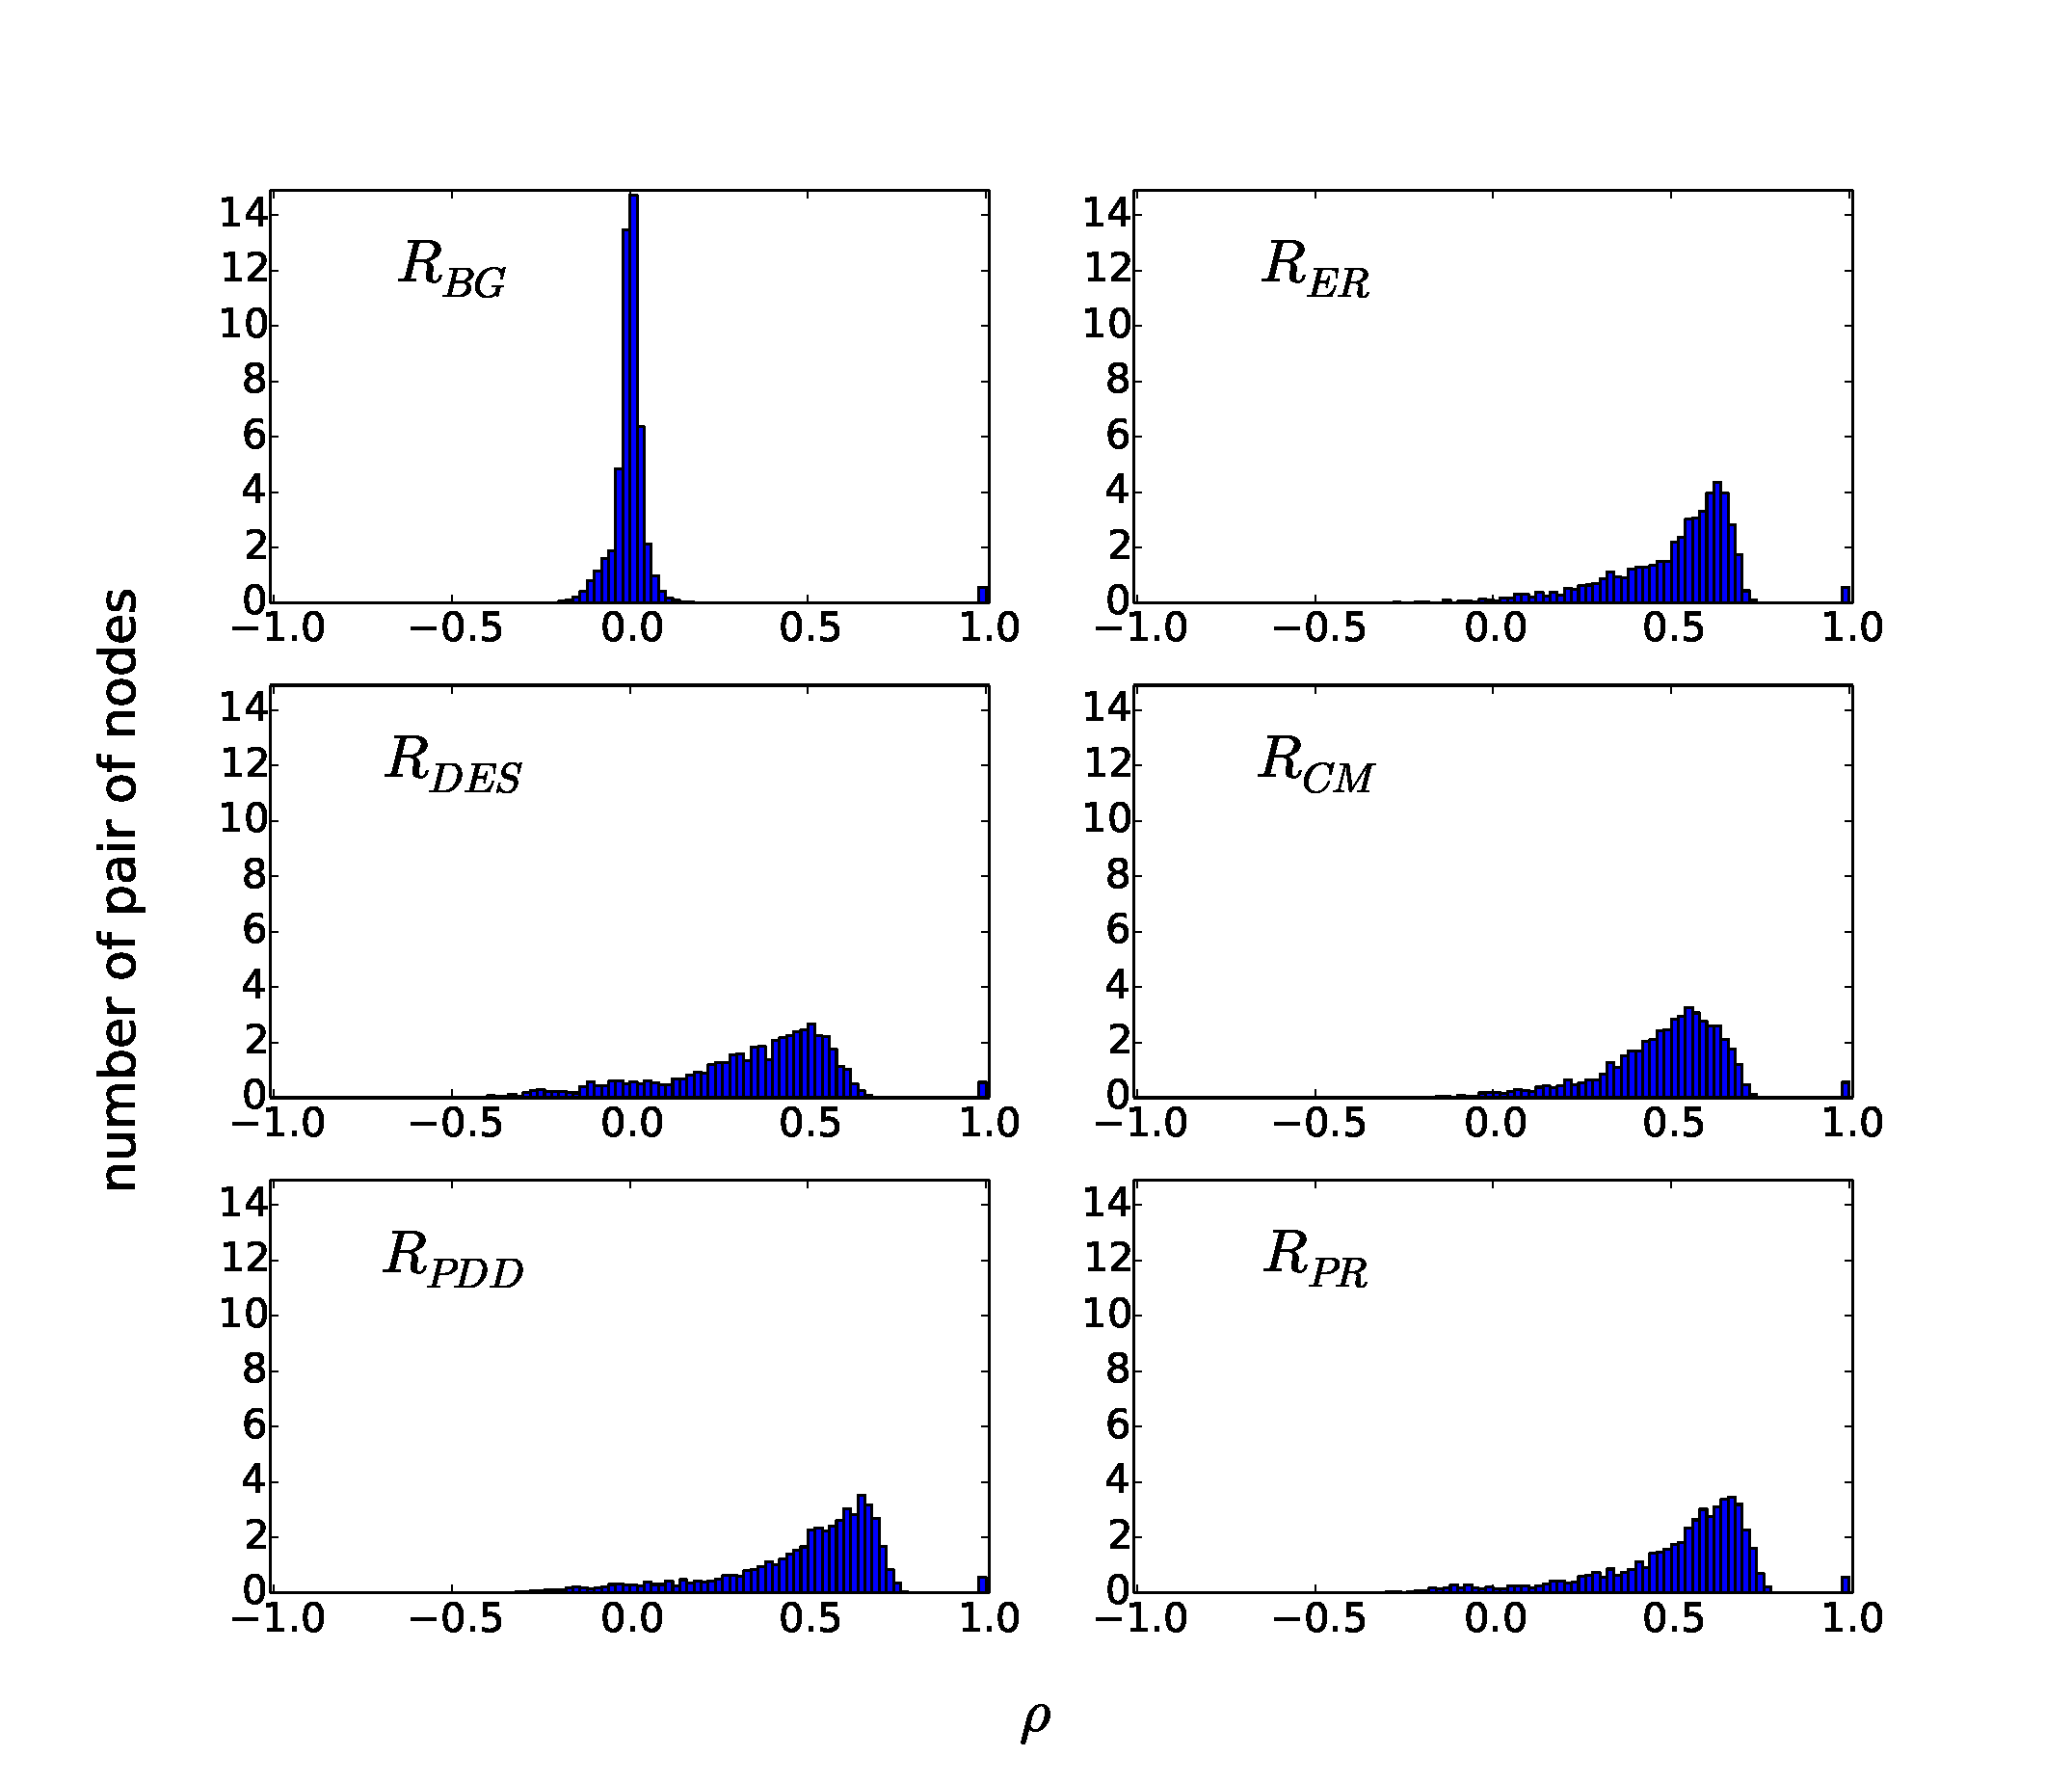
\includegraphics[width=\textwidth]{Figures/Random_ACM_histo.eps}
	 \rule{35em}{0.5pt}
  \caption[Histogram Comparison, ACM]{Histograms for the  distributions of $\rho$ among all pairwise combinations of nodal time-series in AC map related graphs (left column, from top to bottom : $R_{BG}$, $R_{DES}$, $R_{PDD}$, right column, from top to bottom: $R_{ER}$, $R_{CM}$, $R_{PR}$).  The FHN network model parameters for the chosen graphs are $c=0.02$, $v=6$ m/s, network topology parameter $p=0.58$. } 
    \label{fig:Histogram Comparison, ACM}
\end{figure}  

Figure 3.18 illustrates an exemplary set of histograms of $\rho$ values for the $R_{BG}$, which is constructed on an AM obtained at $p=0.58$ and five random graphs, which are built by manipulating this AM via randomization tools provided by \textsc{NetworX} and \textsc{BCT} algorithms (Section 2.3) \citep{XYZNETW, XYZBCT}. The parameters of the neuronal time-series are the coupling strength $c=0.02$ and the signal propagation velocity along axons $v=6$ m/s.   

The frequency of $\rho$ values in $R_{BG}$ resembles a normal distribution around mean 0, indicating the dominance of non-correlated node pairs in terms of their modeled temporal dynamics. All random networks tend to have correlated time-series around $\rho=0.5$ the most frequently, and they exhibit almost no anti-correlation. The peaks at $\rho =1.0$ in each graph corresponds to self-paired nodes, i.e. $\rho_{i,i}=1.0$ for node $i$.  



\begin{figure}[htbp]
 
  \centering

	 \includegraphics[width=\textwidth]{Figures/Random_ACM_PA.eps}

	  \rule{35em}{0.5pt}  
  \caption[Random Graph Comparison, ACM]{ Each heat map corresponds to statistical comparison of brain graph to random graphs in terms of FHN network modeled time-series (left column, from top to bottom: $d(H_{BG}, H_{ER})$, $d(H_{BG}, H_{CM})$, $d(H_{BG}, H_{PR})$, right column, from top to bottom: $d(H_{BG}, H_{DES})$, $d(H_{BG}, H_{PDD})$). }
    \label{fig:Random Graph Comparison, ACM}
 	
\end{figure}  


Figure 3.19 represents the Bhattacharya coefficients $d(H_b,H_r)$ between the AC related brain  graph and five types of random networks, i.e.  $d(H_{BG}, H_{ER})$, $d(H_{BG}, H_{CM})$, $d(H_{BG}, H_{PR})$ $d(H_{BG}, H_{DES})$, $d(H_{BG}, H_{PDD})$. The colorbars express the magnitude of $d(H_b,H_r)$. The hot colors indicate a diversity between $R_{BG}$ and the random graph, whereas the cold colors denote an analogy. 

The anatomical connectivity map related brain graph $R_{BG}$ and its randomized networks are clearly distinguishable at $ 0.38 \leq p \leq 0.7$ and at low $c$-values 0.1, 0.05, 0.02. The $p$-range corresponds to a network density of $ 0.18 \geq \kappa \geq 0.15 $ for all AC related graphs (Section 2.4.1). The network topology of random networks $R_{ER}$, $R_{DES}$, $R_{PDD}$, $R_{CM}$, $R_{PR}$ are quite similar to each other in this $\kappa$-range (Section 2.4, Appendix B). However, the network properties of $R_{BG}$ are distinct from random networks. This diversity can be preserved in terms of temporal dynamics of network types at low coupling strength $c$, meaning small scaled FHN oscillations. 

At $1 \geq p>0.7$, the topology of $R_{BG}$ begin to change dramatically, shortest pathway $d_{ij}$ and small worldness $S$ increases suddenly, global and local efficiency drops to zero (Appendix B). In terms of modeled temporal brain dynamics, $R_{BG}$ above $p>0.7$ becomes less different than random graphs, especially at large scale oscillating brain nodes at $c>0.1$.  
 
This section demonstrated that the FHN network model on anatomical brain graph makes it possible to distinguish the neuronal time-series of $R_{BG}$ from that of random networks. This proposal was also captured for the functional brain graphs in the previous section. 


 